%------Document Class------------
\pdfminorversion=4
\documentclass[10pt,xcolor=dvipsnames]{beamer}
\makeatletter\let\ifGm@compatii\relax\makeatother %workaround to enforce compatibility of different versions of the

%------Usepackage------------
\usepackage[ngerman]{babel}
\usepackage[utf8]{inputenc}
%\usepackage[T1]{fontenc}
\usepackage{lmodern}

\usepackage{amsmath} %
\usepackage{mathtools}
\usepackage{mathrsfs}
\usepackage{dsfont}  
\usepackage{amssymb}
\usepackage{appendixnumberbeamer}
\usepackage[backend=biber,
			style=alphabetic,
			sortlocale=de_DE,
			natbib=true,
			url=false, 
			doi=true,
			eprint=false
			]{biblatex}


\usepackage{caption}
\usepackage{blindtext}
\usepackage{multicol}
\usepackage{wrapfig}
\usepackage{graphicx}
\usepackage{eurosym}
\usepackage{url}
\usepackage{booktabs} 
\usepackage{epstopdf}
\usepackage{pgf,tikz}
\usepackage{xargs}                      % Use more than one optional parameter in a new commands
\usepackage[dvipsnames]{xcolor}  
\usepackage{epstopdf}
\usepackage{etoolbox}
\usepackage{mdframed}
%\usepackage{hyperref}
\usepackage{amsthm}
\usepackage{colortbl}
\usepackage{pgf}
\usepackage{subfigure}
\usepackage{chemformula}
\usepackage[
	per=frac,
	fraction=nice,
	decimalsymbol=comma,
	binary-units=true,
	loctolang={DE:ngerman,UK:english},
]{siunitx}
\usepackage{thmtools}
\newcommand\bmmax{0}
\usepackage{bm}
\usepackage[Symbolsmallscale]{upgreek}
\usepackage{fixmath}
%%% Doc: ftp://tug.ctan.org/pub/tex-archive/macros/latex/contrib/pdfpages/pdfpages.pdf
\usepackage{pdfpages} % Include pages from external PDF documents in LaTeX documents
\usepackage{longtable}
\usepackage{tabularx}
\usepackage{adjustbox}
\usepackage[normalem]{ulem}
\usepackage[colorinlistoftodos,prependcaption,textsize=tiny]{todonotes}
\presetkeys{todonotes}{inline}{}
\newcommandx{\info}[2][1=]{\todo[linecolor=OliveGreen,backgroundcolor=OliveGreen!25,bordercolor=OliveGreen,#1]{#2}}

%------Navigation List on/off------------
\setbeamertemplate{navigation symbols}{}

%------Definition insertframetitle------------
\def\insertframetitle{}

\addto{\captionsngerman}{%
	\renewcommand*{\figurename}{Abb.}
	\renewcommand*{\tablename}{Tab.}
}


%------------------------------------------------------------------------
% Grafiken
%\usepackage{pstricks-add}
\usepackage{tikz}
\usepackage{circuitikz}
\usepackage{csvsimple}
\ctikzset{voltage/distance from node=.5}% in \pgf@circ@Rlen units 
\ctikzset{voltage/distance from line=.25}% pos. between 0 and 1 
\ctikzset{voltage/bump b/.initial=1.5}% 
 
%\usepackage{trfsigns}
 
\usepackage{pgfplots}
\usetikzlibrary{plotmarks,math,positioning,shapes,arrows,backgrounds,circuits.logic.IEC,circuits.ee.IEC,decorations.pathmorphing,patterns,shapes.misc,shapes.geometric,calc,fit,spy,matrix,tikzmark}

%% NUR unter Windows mit texlive notwendig
\makeatletter
\global\let\tikz@ensure@dollar@catcode=\relax

\newcommand{\symbolbegr}{
\begin{tikzpicture}
	\draw[black] (0,0)--(0.2,0)--(0.8,1)--(1,1);
	\draw[black,->] (0,0.5)--(1,0.5);
	\draw[black,->] (0.5,0)--(0.5,1);
\end{tikzpicture}
}

\newcommand{\symbolhyst}{
\begin{tikzpicture}
	\draw[black,->] (0,0.2)--(0.8,0.2)--(0.8,0.8);
	\draw[black,<-] (0.2,0.2)--(0.2,0.8)--(1,0.8);
	
	\draw[black,->] (0,0.5)--(1,0.5);
	\draw[black,->] (0.5,0)--(0.5,1);
\end{tikzpicture}
}

\pgfdeclarepatternformonly{north east lines wide}%
   {\pgfqpoint{-1pt}{-1pt}}%
   {\pgfqpoint{10pt}{10pt}}%
   {\pgfqpoint{9pt}{9pt}}%
   {
     \pgfsetlinewidth{0.4pt}
     \pgfpathmoveto{\pgfqpoint{0pt}{0pt}}
     \pgfpathlineto{\pgfqpoint{9.1pt}{9.1pt}}
     \pgfusepath{stroke}
    }

\pgfdeclarepatternformonly{north west lines wide}%
   {\pgfqpoint{-1pt}{-1pt}}%
   {\pgfqpoint{10pt}{10pt}}%
   {\pgfqpoint{9pt}{9pt}}%
   {
     \pgfsetlinewidth{0.4pt}
     \pgfpathmoveto{\pgfqpoint{0pt}{9.1pt}}
     \pgfpathlineto{\pgfqpoint{9.1pt}{0pt}}
     \pgfusepath{stroke}
    }

\pgfkeys{/pgf/.cd,
  parallelepiped offset x/.initial=2mm,
  parallelepiped offset y/.initial=2mm
}
\pgfdeclareshape{parallelepiped}
{
  \inheritsavedanchors[from=rectangle] % this is nearly a rectangle
  \inheritanchorborder[from=rectangle]
  \inheritanchor[from=rectangle]{north}
  \inheritanchor[from=rectangle]{north west}
  \inheritanchor[from=rectangle]{north east}
  \inheritanchor[from=rectangle]{center}
  \inheritanchor[from=rectangle]{west}
  \inheritanchor[from=rectangle]{east}
  \inheritanchor[from=rectangle]{mid}
  \inheritanchor[from=rectangle]{mid west}
  \inheritanchor[from=rectangle]{mid east}
  \inheritanchor[from=rectangle]{base}
  \inheritanchor[from=rectangle]{base west}
  \inheritanchor[from=rectangle]{base east}
  \inheritanchor[from=rectangle]{south}
  \inheritanchor[from=rectangle]{south west}
  \inheritanchor[from=rectangle]{south east}
  \backgroundpath{
    % store lower right in xa/ya and upper right in xb/yb
    \southwest \pgf@xa=\pgf@x \pgf@ya=\pgf@y
    \northeast \pgf@xb=\pgf@x \pgf@yb=\pgf@y
    \pgfmathsetlength\pgfutil@tempdima{\pgfkeysvalueof{/pgf/parallelepiped offset x}}
    \pgfmathsetlength\pgfutil@tempdimb{\pgfkeysvalueof{/pgf/parallelepiped offset y}}
    \def\ppd@offset{\pgfpoint{\pgfutil@tempdima}{\pgfutil@tempdimb}}
    \pgfpathmoveto{\pgfqpoint{\pgf@xa}{\pgf@ya}}
    \pgfpathlineto{\pgfqpoint{\pgf@xb}{\pgf@ya}}
    \pgfpathlineto{\pgfqpoint{\pgf@xb}{\pgf@yb}}
    \pgfpathlineto{\pgfqpoint{\pgf@xa}{\pgf@yb}}
    \pgfpathclose
    \pgfpathmoveto{\pgfqpoint{\pgf@xb}{\pgf@ya}}
    \pgfpathlineto{\pgfpointadd{\pgfpoint{\pgf@xb}{\pgf@ya}}{\ppd@offset}}
    \pgfpathlineto{\pgfpointadd{\pgfpoint{\pgf@xb}{\pgf@yb}}{\ppd@offset}}
    \pgfpathlineto{\pgfpointadd{\pgfpoint{\pgf@xa}{\pgf@yb}}{\ppd@offset}}
    \pgfpathlineto{\pgfqpoint{\pgf@xa}{\pgf@yb}}
    \pgfpathmoveto{\pgfqpoint{\pgf@xb}{\pgf@yb}}
    \pgfpathlineto{\pgfpointadd{\pgfpoint{\pgf@xb}{\pgf@yb}}{\ppd@offset}}
  }
}

\pgfdeclareshape{zohswitch}{
  \inheritsavedanchors[from=rectangle]
  \inheritanchorborder[from=rectangle]
  \inheritanchor[from=rectangle]{center}
  \inheritanchor[from=rectangle]{base}
  \inheritanchor[from=rectangle]{north}
  \inheritanchor[from=rectangle]{north east}
  \inheritanchor[from=rectangle]{east}
  \inheritanchor[from=rectangle]{south east}
  \inheritanchor[from=rectangle]{south}
  \inheritanchor[from=rectangle]{south west}
  \inheritanchor[from=rectangle]{west}
  \inheritanchor[from=rectangle]{north west}
  \behindbackgroundpath{
    %  store lower right in xa/ya and upper right in xb/yb
    \southwest \pgf@xa=\pgf@x \pgf@ya=\pgf@y
    \northeast \pgf@xb=\pgf@x \pgf@yb=\pgf@y
    
    \pgfpathmoveto{\pgfpoint{\pgf@xa}{(\pgf@ya + \pgf@yb)/2}}
    %\pgfpathlineto{\pgfpoint{(\pgf@xa + \pgf@xb)/4}{(\pgf@ya + \pgf@yb)/2}}
    \pgfpathlineto{\pgfpoint{\pgf@xb}{\pgf@yb}}
    %\pgfpathmoveto{\pgfpoint{\pgf@xa + \pgf@xb)* 3 / 4 }{(\pgf@ya + \pgf@yb)/2}}
    %\pgfpathlineto{\pgfpoint{\pgf@xb}{(\pgf@ya + \pgf@yb)/2}}
    
    \pgfsetlinewidth{.15mm}\pgfsetarrows{-}\pgfsetstrokecolor{black}\pgfusepath{stroke}
 }
}

\pgfdeclareshape{datastore}{
  \inheritsavedanchors[from=rectangle]
  \inheritanchorborder[from=rectangle]
  \inheritanchor[from=rectangle]{center}
  \inheritanchor[from=rectangle]{base}
  \inheritanchor[from=rectangle]{north}
  \inheritanchor[from=rectangle]{north east}
  \inheritanchor[from=rectangle]{east}
  \inheritanchor[from=rectangle]{south east}
  \inheritanchor[from=rectangle]{south}
  \inheritanchor[from=rectangle]{south west}
  \inheritanchor[from=rectangle]{west}
  \inheritanchor[from=rectangle]{north west}
%  \behindbackgroundpath{
    %  store lower right in xa/ya and upper right in xb/yb
%    \southwest \pgf@xa=\pgf@x \pgf@ya=\pgf@y
%    \northeast \pgf@xb=\pgf@x \pgf@yb=\pgf@y
%    \pgfpathmoveto{\pgfpoint{\pgf@xa}{\pgf@ya}}
%    \pgfpathlineto{\pgfpoint{\pgf@xb}{\pgf@ya}}
%    \pgfpathmoveto{\pgfpoint{\pgf@xa}{\pgf@yb}}
%    \pgfpathlineto{\pgfpoint{\pgf@xb}{\pgf@yb}}

    % Draw it, always black, arrowless and .5mm width
%    \pgfsetlinewidth{.5mm}\pgfsetarrows{-}\pgfsetstrokecolor{black}\pgfusepath{stroke}
% }
  \backgroundpath{
    %  store lower right in xa/ya and upper right in xb/yb
    \southwest \pgf@xa=\pgf@x \pgf@ya=\pgf@y
    \northeast \pgf@xb=\pgf@x \pgf@yb=\pgf@y
    \pgfpathmoveto{\pgfpoint{\pgf@xa}{\pgf@ya}}
    \pgfpathlineto{\pgfpoint{\pgf@xb}{\pgf@ya}}
    \pgfpathmoveto{\pgfpoint{\pgf@xa}{\pgf@yb}}
    \pgfpathlineto{\pgfpoint{\pgf@xb}{\pgf@yb}}
 }
}

% coilup, coildown decorations
% code by Hans-Peter E. Kristiansen
% in http://tex.stackexchange.com/a/43605/3954
% Parameters: \pgfdecorationsegmentamplitude, \pgfdecorationsegmentlength,

\pgfdeclaredecoration{coilup}{coil}
{
  \state{coil}[switch if less than=%
    1.5\pgfdecorationsegmentlength+%
    \pgfdecorationsegmentaspect\pgfdecorationsegmentamplitude+%
    \pgfdecorationsegmentaspect\pgfdecorationsegmentamplitude to last,
               width=+\pgfdecorationsegmentlength]
  {
    \pgfpathcurveto
    {\pgfpoint@oncoil{0    }{ 0.555}{1}}
    {\pgfpoint@oncoil{0.445}{ 1    }{2}}
    {\pgfpoint@oncoil{1    }{ 1    }{3}}
    \pgfpathmoveto{\pgfpoint@oncoil{1    }{-1    }{9}}
    \pgfpathcurveto
    {\pgfpoint@oncoil{0.445}{-1    }{10}}
    {\pgfpoint@oncoil{0    }{-0.555}{11}}
    {\pgfpoint@oncoil{0    }{ 0    }{12}}
  }
  \state{last}[width=.5\pgfdecorationsegmentlength+%
    \pgfdecorationsegmentaspect\pgfdecorationsegmentamplitude+%
    \pgfdecorationsegmentaspect\pgfdecorationsegmentamplitude,next state=final]
  {
    \pgfpathcurveto
    {\pgfpoint@oncoil{0    }{ 0.555}{1}}
    {\pgfpoint@oncoil{0.445}{ 1    }{2}}
    {\pgfpoint@oncoil{1    }{ 1    }{3}}
    \pgfpathmoveto{\pgfpoint@oncoil{2    }{ 0    }{6}}
  }
  \state{final}
  {
  \pgfpathmoveto{\pgfpointdecoratedpathlast}
  }
}


% coildown decoration
%
% Parameters: \pgfdecorationsegmentamplitude, \pgfdecorationsegmentlength,

\pgfdeclaredecoration{coildown}{coil}
{
  \state{coil}[switch if less than=%
    1.5\pgfdecorationsegmentlength+%
    \pgfdecorationsegmentaspect\pgfdecorationsegmentamplitude+%
    \pgfdecorationsegmentaspect\pgfdecorationsegmentamplitude to last,
               width=+\pgfdecorationsegmentlength]
  {
    \pgfpathmoveto{\pgfpoint@oncoil{1    }{1    }{3}}
    \pgfpathcurveto
    {\pgfpoint@oncoil{1.555}{ 1    }{4}}
    {\pgfpoint@oncoil{2    }{ 0.555}{5}}
    {\pgfpoint@oncoil{2    }{ 0    }{6}}
    \pgfpathcurveto
    {\pgfpoint@oncoil{2    }{-0.555}{7}}
    {\pgfpoint@oncoil{1.555}{-1    }{8}}
    {\pgfpoint@oncoil{1    }{-1    }{9}}
  }
  \state{last}[width=.5\pgfdecorationsegmentlength+%
    \pgfdecorationsegmentaspect\pgfdecorationsegmentamplitude+%
    \pgfdecorationsegmentaspect\pgfdecorationsegmentamplitude,next state=final]
  {
    \pgfpathmoveto{\pgfpoint@oncoil{1    }{ 1    }{3}}
    \pgfpathcurveto
    {\pgfpoint@oncoil{1.555}{ 1    }{4}}
    {\pgfpoint@oncoil{2    }{ 0.555}{5}}
    {\pgfpoint@oncoil{2    }{ 0    }{6}}
  }
  \state{final}
  {
  \pgfpathlineto{\pgfpointdecoratedpathlast}
  }
}

\def\pgfpoint@oncoil#1#2#3{%
  \pgf@x=#1\pgfdecorationsegmentamplitude%
  \pgf@x=\pgfdecorationsegmentaspect\pgf@x%
  \pgf@y=#2\pgfdecorationsegmentamplitude%
  \pgf@xa=0.083333333333\pgfdecorationsegmentlength%
  \advance\pgf@x by#3\pgf@xa%
}

% definition of error function
\pgfmathdeclarefunction{erf}{1}{%
  \begingroup
    \pgfmathparse{#1 > 0 ? 1 : -1}%
    \edef\sign{\pgfmathresult}%
    \pgfmathparse{abs(#1)}%
    \edef\x{\pgfmathresult}%
    \pgfmathparse{1/(1+0.3275911*\x)}%
    \edef\t{\pgfmathresult}%
    \pgfmathparse{%
      1 - (((((1.061405429*\t -1.453152027)*\t) + 1.421413741)*\t 
      -0.284496736)*\t + 0.254829592)*\t*exp(-(\x*\x))}%
    \edef\y{\pgfmathresult}%
    \pgfmathparse{(\sign)*\y}%
    \pgfmath@smuggleone\pgfmathresult%
  \endgroup
}

\newif\ifcuboidshade
\newif\ifcuboidemphedge

\tikzset{
  cuboid/.is family,
  cuboid,
  shiftx/.initial=0,
  shifty/.initial=0,
  dimx/.initial=3,
  dimy/.initial=3,
  dimz/.initial=3,
  scale/.initial=1,
  densityx/.initial=1,
  densityy/.initial=1,
  densityz/.initial=1,
  rotation/.initial=0,
  anglex/.initial=0,
  angley/.initial=90,
  anglez/.initial=225,
  scalex/.initial=1,
  scaley/.initial=1,
  scalez/.initial=0.5,
  front/.style={draw=black,fill=white},
  top/.style={draw=black,fill=white},
  right/.style={draw=black,fill=white},
  shade/.is if=cuboidshade,
  shadecolordark/.initial=black,
  shadecolorlight/.initial=white,
  shadeopacity/.initial=0.15,
  shadesamples/.initial=16,
  emphedge/.is if=cuboidemphedge,
  emphstyle/.style={thick},
}

\newcommand{\tikzcuboidkey}[1]{\pgfkeysvalueof{/tikz/cuboid/#1}}

% Commands
\newcommand\sidecomment[5][0.1]%
  {\begin{tikzpicture}[remember picture,overlay]
   \draw[-stealth]
     ($({pic cs:#4}|-{pic cs:#2})+(#1,0)$)
     .. controls +(0.2,-0.05) and +(0.2,0.1) ..
     node[right,align=left]{#5}
     ($({pic cs:#4}|-{pic cs:#3})+(#1,0.1)$);
   \end{tikzpicture}%
  }

\newcommand{\tikzcuboid}[1]{
    \tikzset{cuboid,#1} % Process Keys passed to command
  \pgfmathsetlengthmacro{\vectorxx}{\tikzcuboidkey{scalex}*cos(\tikzcuboidkey{anglex})*28.452756}
  \pgfmathsetlengthmacro{\vectorxy}{\tikzcuboidkey{scalex}*sin(\tikzcuboidkey{anglex})*28.452756}
  \pgfmathsetlengthmacro{\vectoryx}{\tikzcuboidkey{scaley}*cos(\tikzcuboidkey{angley})*28.452756}
  \pgfmathsetlengthmacro{\vectoryy}{\tikzcuboidkey{scaley}*sin(\tikzcuboidkey{angley})*28.452756}
  \pgfmathsetlengthmacro{\vectorzx}{\tikzcuboidkey{scalez}*cos(\tikzcuboidkey{anglez})*28.452756}
  \pgfmathsetlengthmacro{\vectorzy}{\tikzcuboidkey{scalez}*sin(\tikzcuboidkey{anglez})*28.452756}
  \begin{scope}[xshift=\tikzcuboidkey{shiftx}, yshift=\tikzcuboidkey{shifty}, scale=\tikzcuboidkey{scale}, rotate=\tikzcuboidkey{rotation}, x={(\vectorxx,\vectorxy)}, y={(\vectoryx,\vectoryy)}, z={(\vectorzx,\vectorzy)}]
    \pgfmathsetmacro{\steppingx}{1/\tikzcuboidkey{densityx}}
  \pgfmathsetmacro{\steppingy}{1/\tikzcuboidkey{densityy}}
  \pgfmathsetmacro{\steppingz}{1/\tikzcuboidkey{densityz}}
  \newcommand{\dimx}{\tikzcuboidkey{dimx}}
  \newcommand{\dimy}{\tikzcuboidkey{dimy}}
  \newcommand{\dimz}{\tikzcuboidkey{dimz}}
  \pgfmathsetmacro{\secondx}{2*\steppingx}
  \pgfmathsetmacro{\secondy}{2*\steppingy}
  \pgfmathsetmacro{\secondz}{2*\steppingz}
  \foreach \x in {\steppingx,\secondx,...,\dimx}
  { \foreach \y in {\steppingy,\secondy,...,\dimy}
    {   \pgfmathsetmacro{\lowx}{(\x-\steppingx)}
      \pgfmathsetmacro{\lowy}{(\y-\steppingy)}
      \filldraw[cuboid/front] (\lowx,\lowy,\dimz) -- (\lowx,\y,\dimz) -- (\x,\y,\dimz) -- (\x,\lowy,\dimz) -- cycle;
    }
    }
  \foreach \x in {\steppingx,\secondx,...,\dimx}
  { \foreach \z in {\steppingz,\secondz,...,\dimz}
    {   \pgfmathsetmacro{\lowx}{(\x-\steppingx)}
      \pgfmathsetmacro{\lowz}{(\z-\steppingz)}
      \filldraw[cuboid/top] (\lowx,\dimy,\lowz) -- (\lowx,\dimy,\z) -- (\x,\dimy,\z) -- (\x,\dimy,\lowz) -- cycle;
        }
    }
    \foreach \y in {\steppingy,\secondy,...,\dimy}
  { \foreach \z in {\steppingz,\secondz,...,\dimz}
    {   \pgfmathsetmacro{\lowy}{(\y-\steppingy)}
      \pgfmathsetmacro{\lowz}{(\z-\steppingz)}
      \filldraw[cuboid/right] (\dimx,\lowy,\lowz) -- (\dimx,\lowy,\z) -- (\dimx,\y,\z) -- (\dimx,\y,\lowz) -- cycle;
    }
  }
  \ifcuboidemphedge
    \draw[cuboid/emphstyle] (0,\dimy,0) -- (\dimx,\dimy,0) -- (\dimx,\dimy,\dimz) -- (0,\dimy,\dimz) -- cycle;%
    \draw[cuboid/emphstyle] (0,\dimy,\dimz) -- (0,0,\dimz) -- (\dimx,0,\dimz) -- (\dimx,\dimy,\dimz);%
    \draw[cuboid/emphstyle] (\dimx,\dimy,0) -- (\dimx,0,0) -- (\dimx,0,\dimz);%
    \fi

    \ifcuboidshade
    \pgfmathsetmacro{\cstepx}{\dimx/\tikzcuboidkey{shadesamples}}
    \pgfmathsetmacro{\cstepy}{\dimy/\tikzcuboidkey{shadesamples}}
    \pgfmathsetmacro{\cstepz}{\dimz/\tikzcuboidkey{shadesamples}}
    \foreach \s in {1,...,\tikzcuboidkey{shadesamples}}
    {   \pgfmathsetmacro{\lows}{\s-1}
        \pgfmathsetmacro{\cpercent}{(\lows)/(\tikzcuboidkey{shadesamples}-1)*100}
        \fill[opacity=\tikzcuboidkey{shadeopacity},color=\tikzcuboidkey{shadecolorlight}!\cpercent!\tikzcuboidkey{shadecolordark}] (0,\s*\cstepy,\dimz) -- (\s*\cstepx,\s*\cstepy,\dimz) -- (\s*\cstepx,0,\dimz) -- (\lows*\cstepx,0,\dimz) -- (\lows*\cstepx,\lows*\cstepy,\dimz) -- (0,\lows*\cstepy,\dimz) -- cycle;
        \fill[opacity=\tikzcuboidkey{shadeopacity},color=\tikzcuboidkey{shadecolorlight}!\cpercent!\tikzcuboidkey{shadecolordark}] (0,\dimy,\s*\cstepz) -- (\s*\cstepx,\dimy,\s*\cstepz) -- (\s*\cstepx,\dimy,0) -- (\lows*\cstepx,\dimy,0) -- (\lows*\cstepx,\dimy,\lows*\cstepz) -- (0,\dimy,\lows*\cstepz) -- cycle;
        \fill[opacity=\tikzcuboidkey{shadeopacity},color=\tikzcuboidkey{shadecolorlight}!\cpercent!\tikzcuboidkey{shadecolordark}] (\dimx,0,\s*\cstepz) -- (\dimx,\s*\cstepy,\s*\cstepz) -- (\dimx,\s*\cstepy,0) -- (\dimx,\lows*\cstepy,0) -- (\dimx,\lows*\cstepy,\lows*\cstepz) -- (\dimx,0,\lows*\cstepz) -- cycle;
    }
    \fi 

  \end{scope}
}

% For spy
\tikzset{
  path picture/.code=\tikz@addmode{\def\tikz@path@picture{#1\tikz@path@picture@extra}},
  path picture extra/.code={\def\tikz@path@picture@extra{#1}}
}
\let\tikz@path@picture@extra\pgfutil@empty

\makeatother

% Dataflows
\tikzstyle{prozess} = [draw, thick, rounded corners, inner sep=.3cm]
\tikzstyle{function} = [draw, thick, circle]
\tikzstyle{ifunction} = [draw, thick, circle split,minimum size=30mm, font=\small]
\tikzstyle{datastore} = [draw, very thick, shape=datastore, inner sep=.3cm]
\tikzstyle{to} = [->, >=stealth', shorten >=1pt, semithick, font=\sffamily\footnotesize]
\tikzstyle{dto} = [->, dashed, >=stealth', shorten >=1pt, semithick, font=\sffamily\footnotesize]
\tikzstyle{wto} = [-, color=white, >=stealth', shorten >=1pt, semithick, font=\sffamily\footnotesize]
\tikzstyle{bto} = [<->, >=stealth', shorten >=1pt, semithick, font=\sffamily\footnotesize]
\tikzstyle{ccircle} = [path picture={ \draw[black] (path picture bounding box.south east) -- (path picture bounding box.north west) (path picture bounding box.south west) -- (path picture bounding box.north east);}]

% Controlflows
\tikzstyle{block} = [draw, fill=white, rectangle, minimum height=3em, minimum width=4em]
\tikzstyle{rblock} = [draw, fill=white, circle, inner sep=0pt,minimum size=1mm]
\tikzstyle{wobblock} = [fill=white, rectangle, minimum height=3em, minimum width=5em]
\tikzstyle{nlblock} = [draw, postaction={draw,line width=0.25mm,white}, line width=0.5mm, black, fill=white, rectangle, minimum height=3em, minimum width=5em]
\tikzstyle{sum} = [draw,circle]
\tikzstyle{branch} = [circle,inner sep=0pt,minimum size=1mm,fill=black,draw=black]
\tikzstyle{nvbranch} = [circle,inner sep=0pt,minimum size=1mm,fill=white,draw=white, fill opacity=0, draw opacity=0]
\tikzstyle{vecBranch} = [circle,inner sep=0pt,minimum size=2mm,fill=black,draw=black]
\tikzstyle{input} = [coordinate]
\tikzstyle{output} = [coordinate] 
\tikzstyle{coord} = [coordinate] 
\tikzstyle{pinstyle} = [pin edge={to-,thin,black}] 
\tikzstyle{vecArrow} = [thick, decoration={markings,mark=at position
   1 with {\arrow[semithick]{open triangle 60}}},
   double distance=1.4pt, shorten >= 5.5pt,
   preaction = {decorate},
   postaction = {draw,line width=1.4pt, white,shorten >= 4.5pt}]
\tikzstyle{vecWithoutArrow} = [thick,
   double distance=1.4pt,
   postaction = {draw,line width=1.4pt, white}]
\tikzset{
  Pfeil/.style={thick,shorten >=#1,shorten <=#1,->,>=latex}, % für Peile
  UPfeil/.style={black,Pfeil=#1,font={\sffamily\itshape}},% für Spannungspfeile
  IPfeil/.style={black,Pfeil=#1,font={\ttfamily\itshape}} % für Strompfeile
}   
\tikzset{cross/.style={cross out, draw=black, minimum size=2*(#1-\pgflinewidth), inner sep=0pt, outer sep=0pt},
%default radius will be 1pt. 
cross/.default={1pt}}

\newcommand*{\rechterWinkel}[3]{% #1 = point, #2 = start angle, #3 = radius
   \draw[shift={(#2:#3)}] (#1) arc[start angle=#2, delta angle=90, radius = #3];
   \fill[shift={(#2+45:#3/2)}] (#1) circle[radius=1.25\pgflinewidth];
}


%%% ----------------------------------------------------------------
% ============================================================
% Definition of mathematic commands
% ============================================================
\renewcommand{\vector}[1]{\left[\begin{array}{c}#1\end{array}\right]}       % vector
\newcommand{\pvector}[1]{\begin{bmatrix} #1 \end{bmatrix}}
\newcommand{\mats}[1]{\ensuremath{\left( \begin{smallmatrix} #1 \end{smallmatrix} \right)}} % small matrix for use in the text
%\renewcommand{\vector}[1]{\begin{array}{*{1}}#1\end{array}}
\renewcommand{\matrix}[2]{\left[\begin{array}{#1}#2\end{array}\right]}      % matrix, \matrix{*{4}{c}}{}
%\renewcommand{\bmatrix}[2]{\left[\begin{array}{#1}#2\end{array}\right]}
% symbol style
%\let\Oldvec\vec \renewcommand{\vec}[1]{\ensuremath{\Oldvec{#1}}}
\newcommand{\mat}[1]{\ensuremath{\mathbf{#1}}}
\let\Oldvec\vec \renewcommand{\vec}[1]{\ensuremath{\boldsymbol{#1}}}
\newcommand{\modulo}[1]{\ensuremath{~~({\rm mod}~#1)}}
\newcommand{\intd}[1]{{\rm d}#1}                     % the d in the integral
\newcommand{\dint}[1]{{\rm d}#1}
\newcommand{\dd}[1]{{\rm d}#1}                     % the d in the integral
\newcommand{\divergence}[1]{{\rm div}(#1)} % divergence
\newcommand{\dotp}[2]{<#1,#2>}
\newcommand{\ident}{\mat{I}}                     % identity matrix
\newcommand{\pderi}[2]{\ensuremath{\frac{\partial #1}{\partial #2}}}                     % partial derivative
\newcommand{\ppderi}[2]{\ensuremath{\frac{\partial^2 #1}{\partial #2^2}}}                     % partial derivative
\newcommand{\deri}[2]{\ensuremath{\frac{{\rm d}#1}{{\rm d}#2}}}                     % partial derivative
%\newcommand{\exp}[1]{exp(#1)}
\newcommand{\laplace}{\ensuremath{\triangle}}                                            % laplace operator
\newcommand{\kroneker}{\ensuremath{\delta_\vartriangle}}                                            % laplace operator
\newcommand{\dirac}{\ensuremath{\delta}}                                            % dirac delta function
\newcommand{\conj}[1][non]{\ensuremath{ \ifthenelse{\equal{#1}{non}}{\ast}{#1^\ast} } }                                            % conjugate complex
\newcommand{\conv}{\ensuremath{\ast}}
\newcommand{\degree}[1][non]{\ensuremath{\ifthenelse{\equal{#1}{non}}{^\circ}{#1^\circ}}}
\newcommand{\I}{\ensuremath{j}}

% alternative symbol for Fourier Transform \mathcal{F}
\newcommand{\FT}[1][non]{\ensuremath{\mathfrak F\ifthenelse{\equal{#1}{non}}{}{ \left\{ #1 \right\}}}}
\newcommand{\IFT}[1][non]{\ensuremath{\mathfrak F^{-1}\ifthenelse{\equal{#1}{non}}{}{ \left\{ #1 \right\} }} }
% usage of the optional parameter: \IFT[f_x] and $\IFT\{f_x\}$ are equivalent and \IFT[non] and \IFT are equivalent
%  \FT[\frac{A^{C^e}}{B}]

\newcommand{\sumsum}[1]{\sum_{i=1}^{n}\sum_{j=1}^{m}{#1}}
\newcommand{\sinc}{\mbox{sinc}}                                             % sinc
\def\sgn{\mathop{\rm sgn}}

%\newcommand{\atan}[1][non]{\tan^{-1}\ensuremath{\ifthenelse{\equal{#1}{non}}{}{ \left( #1 \right)}}}
\newcommand{\atan}[1][non]{\arctan\ensuremath{\ifthenelse{\equal{#1}{non}}{}{ \left( #1 \right)}}}
\newcommand{\tr}[1]{\mbox{tr}\left( #1 \right)}                                                 % trace of an matrix
\renewcommand{\det}[1]{\mbox{det}\left( #1 \right)}                                                 % trace of an matrix
\newcommand{\argmin}[1]{\arg\min_{#1}\ }                            % argmin
\newcommand{\E}[1][non]{\ensuremath{\ifthenelse{\equal{#1}{non}}{E}{E\left\{ #1 \right\}}}}
\newcommand{\N}[3][]{\ensuremath{\mathcal{N}^{#1}(#2,#3)}} % normal distribution
%\newcommand{\chis}[2][]{\ensuremath{\chi^2(#1,#2)}} % chi-sqauare distribution
\newcommand{\chis}[2][non]{\ensuremath{\chi^2 \ifthenelse{\equal{#1}{non}}{}{ \left(#1,#2\right)}}}
\newcommand{\CN}[3][]{\ensuremath{\mathcal{N}_\circ^{#1}(#2,#3)}} % von Mises distribution, circular normal
%\newcommand{\R}[2][xx]{\ensuremath{R_{#1}\left( #2 \right)}} % correlation
\newcommand{\R}[2][xx]{\ensuremath{R_{#1}\ifthenelse{\equal{#2}{}}{}{\left( #2 \right)}}} % correlation
%\newcommand{\S}[2][xx]{\ensuremath{S_{#1}\left( #2 \right)}} % spectral density
\renewcommand{\S}[2][xx]{\ensuremath{S_{#1}\ifthenelse{\equal{#2}{}}{}{\left( #2 \right)}}} % spectral density
\newcommand{\Gammaf}[1][non]{\ensuremath{\Gamma\ifthenelse{\equal{#1}{non}}{}{ \left( #1 \right)}}}
\newcommand{\varrhob}{\overline{\varrho}} % rho bar

%\newcommand{\E}[1][non]{\ensuremath{E\left\{ #1 \right\}}}

\def\mm{\hspace{-1.5mm}\rule[1mm]{1.3mm}{0.15mm}\rule{0.2mm}{0mm}\relax}    % short minus symbol

% Defintionen, Theoreme
\newtheorem{defi}{Definition}
\newtheorem{satz}{Satz}
\newtheorem{hsatz}{Hilfssatz}

\newtheoremstyle{style1} 
   {}                   %Space above 
   {}                   %Space below 
   {}                      %Body font: original {\normalfont} 
   {}                      %Indent amount (empty = no indent, 
                           %\parindent = para indent) 
   {\normalfont\itshape}  %Thm head font original {\normalfont\bfseries} 
   {.}                     %Punctuation after thm head original : 
   { }              %Space after thm head: " " = normal interword 
                           %space; \newline = linebreak 
   {}%\textbf{\thmname{#1}\thmnumber{ #2}\thmnote{ (#3)}}}                     
                                        %Thm head spec (can be left empty, meaning 
                           %`normal') original {\underline{\thmname{#1}\thmnumber{ #2}\thmnote{ (#3)}}} 
  
\newtheoremstyle{style2} 
   {3pt}                   %Space above 
   {3pt}                   %Space below 
   {}                      %Body font: original {\normalfont} 
   {}                      %Indent amount (empty = no indent, 
                           %\parindent = para indent) 
   {\normalfont\bfseries}  %Thm head font original {\normalfont\bfseries} 
   {}                     %Punctuation after thm head original : 
   {\newline}              %Space after thm head: " " = normal interword 
                           %space; \newline = linebreak 
   {\textbf{\thmname{#1}\thmnumber{ #2}\thmnote{ (#3)}}}                     
                                        %Thm head spec (can be left empty, meaning 
                           %`normal') original {\underline{\thmname{#1}\thmnumber{ #2}\thmnote{ (#3)}}} 

\newenvironment{conditions}
  {\par\vspace{\abovedisplayskip}\noindent
   \tabularx{\columnwidth}{>{$}l<{$} @{${}={}$} >{\raggedright\arraybackslash}X}}
  {\endtabularx\par\vspace{\belowdisplayskip}}
 
\newcounter{saveenumi}
\newcommand{\seti}{\setcounter{saveenumi}{\value{enumi}}}
\newcommand{\conti}{\setcounter{enumi}{\value{saveenumi}}}

\newcommand{\footnoteWithoutNum}[1]{
    \renewcommand{\thefootnote}{}
    \footnotetext{\scriptsize#1}
    \renewcommand{\thefootnote}{\arabic{footnote}}
}


\bibliography{./preambel/books}

%------Presentation Mode------------
\newcommand{\pathtostylefile}{}
\mode<presentation> {\usepackage{beamerthemeiace}}

%---------Title,Author,Date----------
\title{3DCSM - Body Handling}
\author{}
\date{}

% My Packages
\usepackage{amsmath,amssymb}
\usepackage{relsize}
\usepackage{graphicx}
\usepackage{media9} 
\usepackage{tikz}
\usepackage[overload]{empheq}
\usetikzlibrary{arrows, matrix, trees, mindmap, positioning}
\usepackage{arydshln}
\usepackage{animate}
\usepackage{anyfontsize}
\newcommand{\tikzfnt}{13}


\begin{document}
%----------------------------------------------------------------------------------------
%	TITLE PAGE
%----------------------------------------------------------------------------------------
{
\setbeamertemplate{footline}{}
\begin{frame}
	\titlepage
\end{frame}
}
\addtocounter{framenumber}{-1}
%----------------------------------------------------------------------------------------
%	PRESENTATION SLIDES
%----------------------------------------------------------------------------------------
\begin{frame}
    %\tableofcontents[hideallsubsections]
    \tableofcontents
\end{frame}

%----------------------------------------------------------------------------------------
%	TABLE OF CONTENTS
%----------------------------------------------------------------------------------------
\AtBeginSection[]{
\begin{frame}
      \tableofcontents[current, currentsubsection]
\end{frame}
}
%----------------------------------------------------------------------------------------
%	PRESENTATION SLIDES
%----------------------------------------------------------------------------------------
\section{Ziel des Arbeitspaketes}
	\begin{frame}{Ziele des Arbeitspaketes}
		\textbf{Erstellen eines dynamischen Modells für das Body-Handling}
		\begin{itemize}
			\item Abbildung des dynamischen Systemverhaltens, statische Aspekte stehen dabei im Hintergund
			\item Das Modell mit Abstraktion des Motors über Momentenvorgabe ist verfügbar
			\item Die um das Motormodell ergänzte Modellstruktur ist fertiggestellt
			\item Die Modelle sind dokumentiert
		\end{itemize}
	\end{frame}

\section{Reduziertes Modell}
	\subsection{Modell mit Parameter}
		\begin{frame}{Ebenes 2d-Modell}
			\begin{itemize}
				\item Ziel: Einfache und möglichst genau dynamische Abbildung des realen Systems
				\item Rechtfertigung für ein ebenes Modell: Kein Freiheitsgrad in x-Richtung
			\end{itemize}
			\begin{minipage}{0.48\textwidth}
				\begin{figure}
					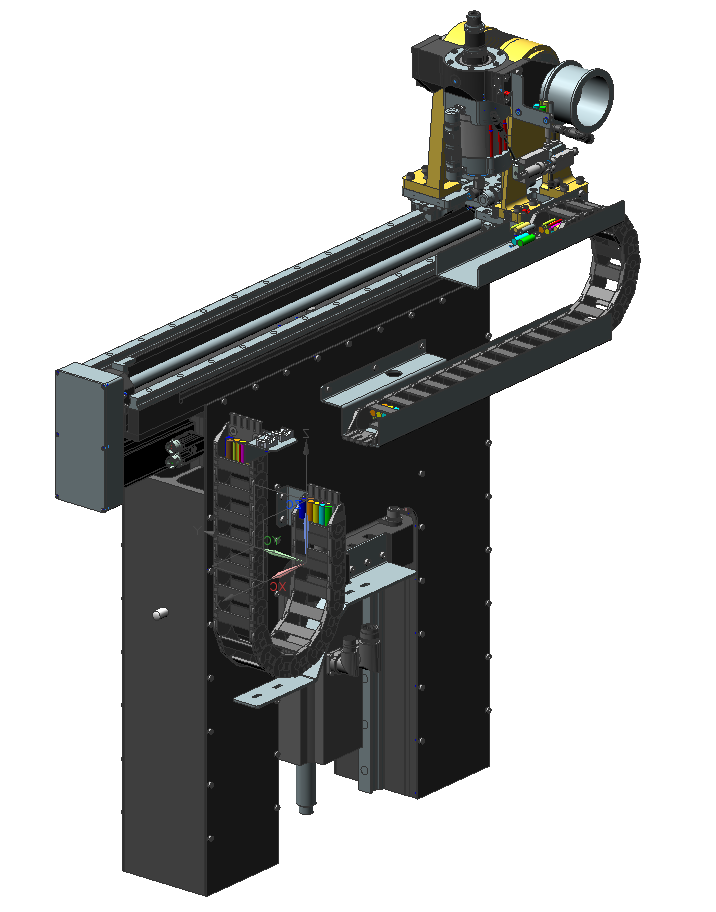
\includegraphics[width=0.9\linewidth]{./pics/aufbau_cad.png}
				\end{figure}
			\end{minipage}
			\hfill
			\begin{minipage}{0.48\textwidth}
				\vspace{-0.2cm}
				\begin{figure}
					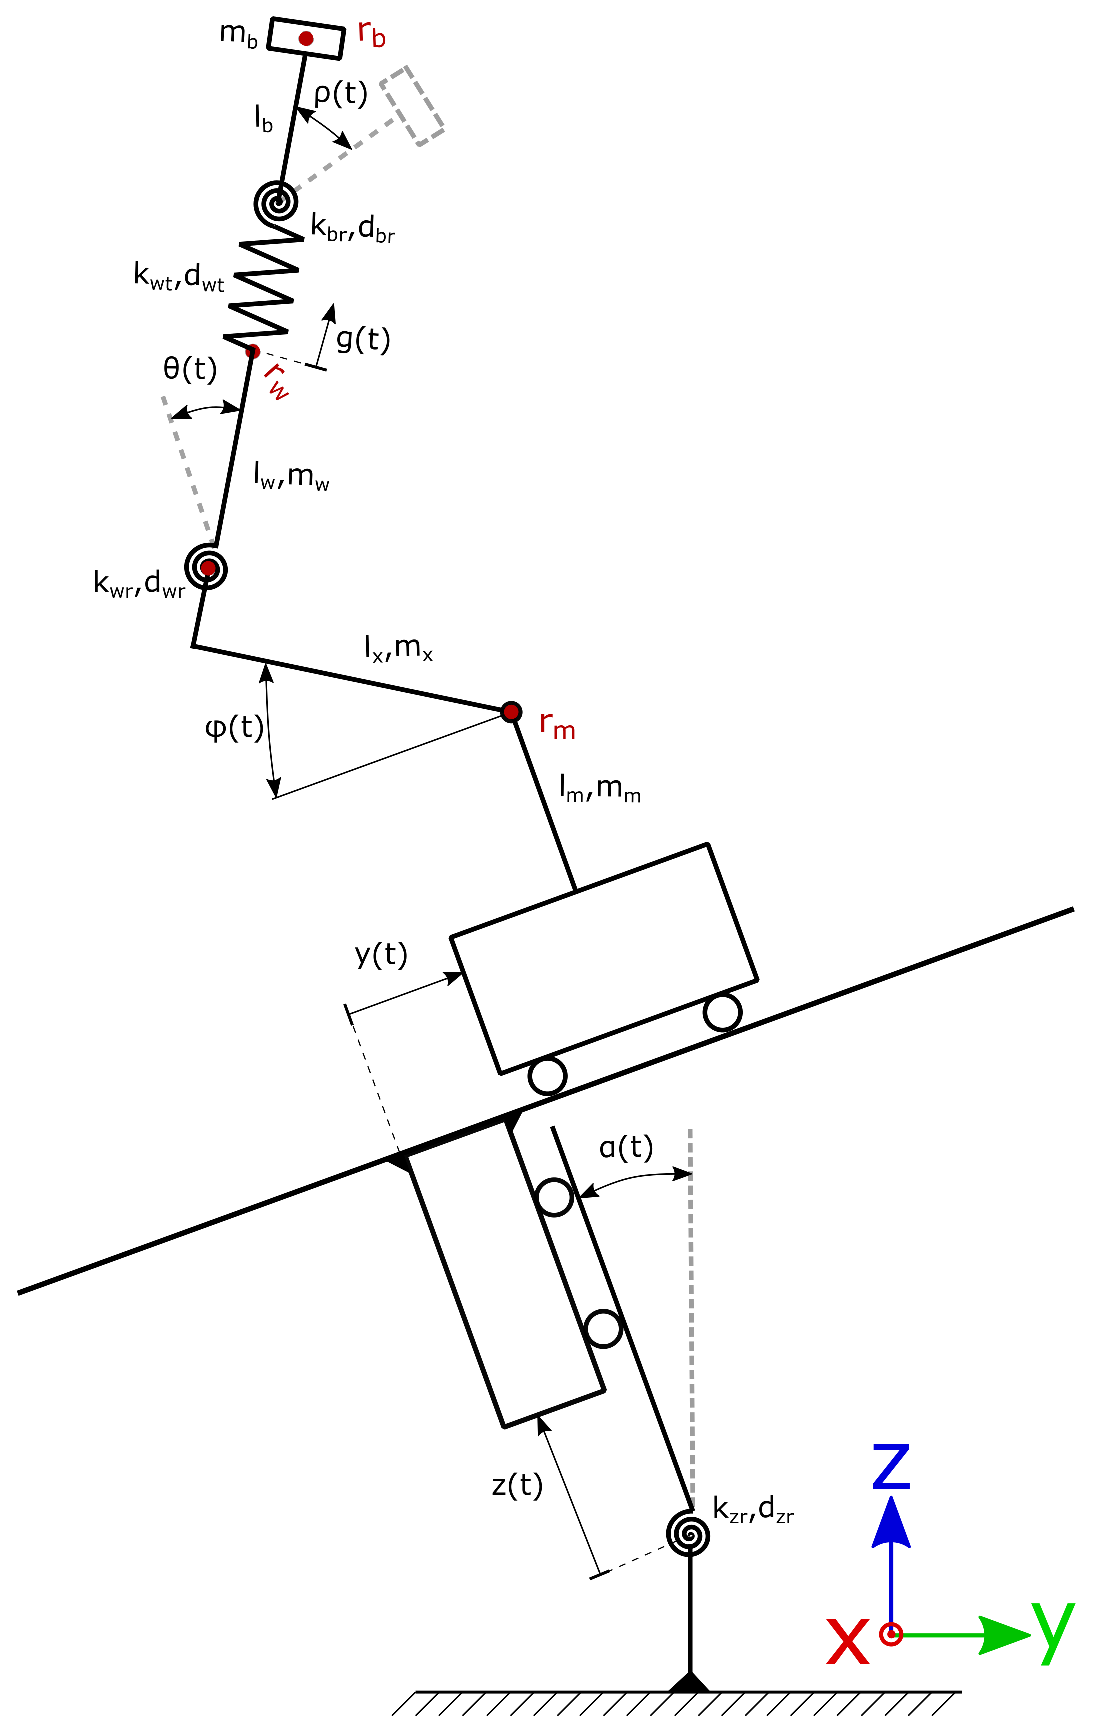
\includegraphics[width=0.7\linewidth]{./pics/SchematischesModell.eps}
				\end{figure}
			\end{minipage}
		\end{frame}

		\begin{frame}{Gesamtmodell}
		\begin{minipage}{0.58\textwidth}
			Generalisierte Koordinaten des Modells
			\[ \bm{q} = [y(t), z(t), \varphi(t), \theta(t), \alpha(t), g(t), \rho(t)]^{T} \]
			Geometrische Parameter in $ m $\\\vspace{10pt} \def\arraystretch{1.2}
			\begin{tabular}{lll}
				$ l_{m}=0.1 $ & $ l_{z}=0.701 $ &  \\ 
				$ l_{x}=0.079 $ & $ l_{w}=0.06 $ & $ l_{b}=0.0286 $\\
			\end{tabular}
			Massen in $ kg $\\\vspace{10pt} \def\arraystretch{1.2}
			\begin{tabular}{lll}
				$ m_{m}=7.62 $ & $ m_{x}=4.87 $ & $ m_{w}=2.37 $   \\ 
				$ m_{b}=0.024 $ & $ m_{z} = 77.3 $ &\\
			\end{tabular}
			Massenträgheitsmomente um X-Achse in $ kgm^{2} $\\\vspace{10pt} \def\arraystretch{1.2}
			\begin{tabular}{lll}
				$ J_{x}=0.0126 $ & $ J_{w}=0.0138 $ & $ J_{y} = 0.063 $ \\ 
				$ J_{b}=0.0000077 $  & $ J_{z}=7.191 $&  \\
			\end{tabular}
			Federkonstanten\\\vspace{10pt} \def\arraystretch{1.3}
			\begin{tabular}{ll}
				$ k_{wr}=217.19\frac{kNm}{rad} $ & $ k_{br}=34.9\frac{kNm}{rad} $ \\ 
				$ k_{wt}=6069\frac{kN}{m} $ & $ k_{zr}=2902.4\frac{kNm}{rad} $ \\   
			\end{tabular}
		\end{minipage}
		\hfill
		\begin{minipage}{0.38\textwidth}
			\begin{figure}
				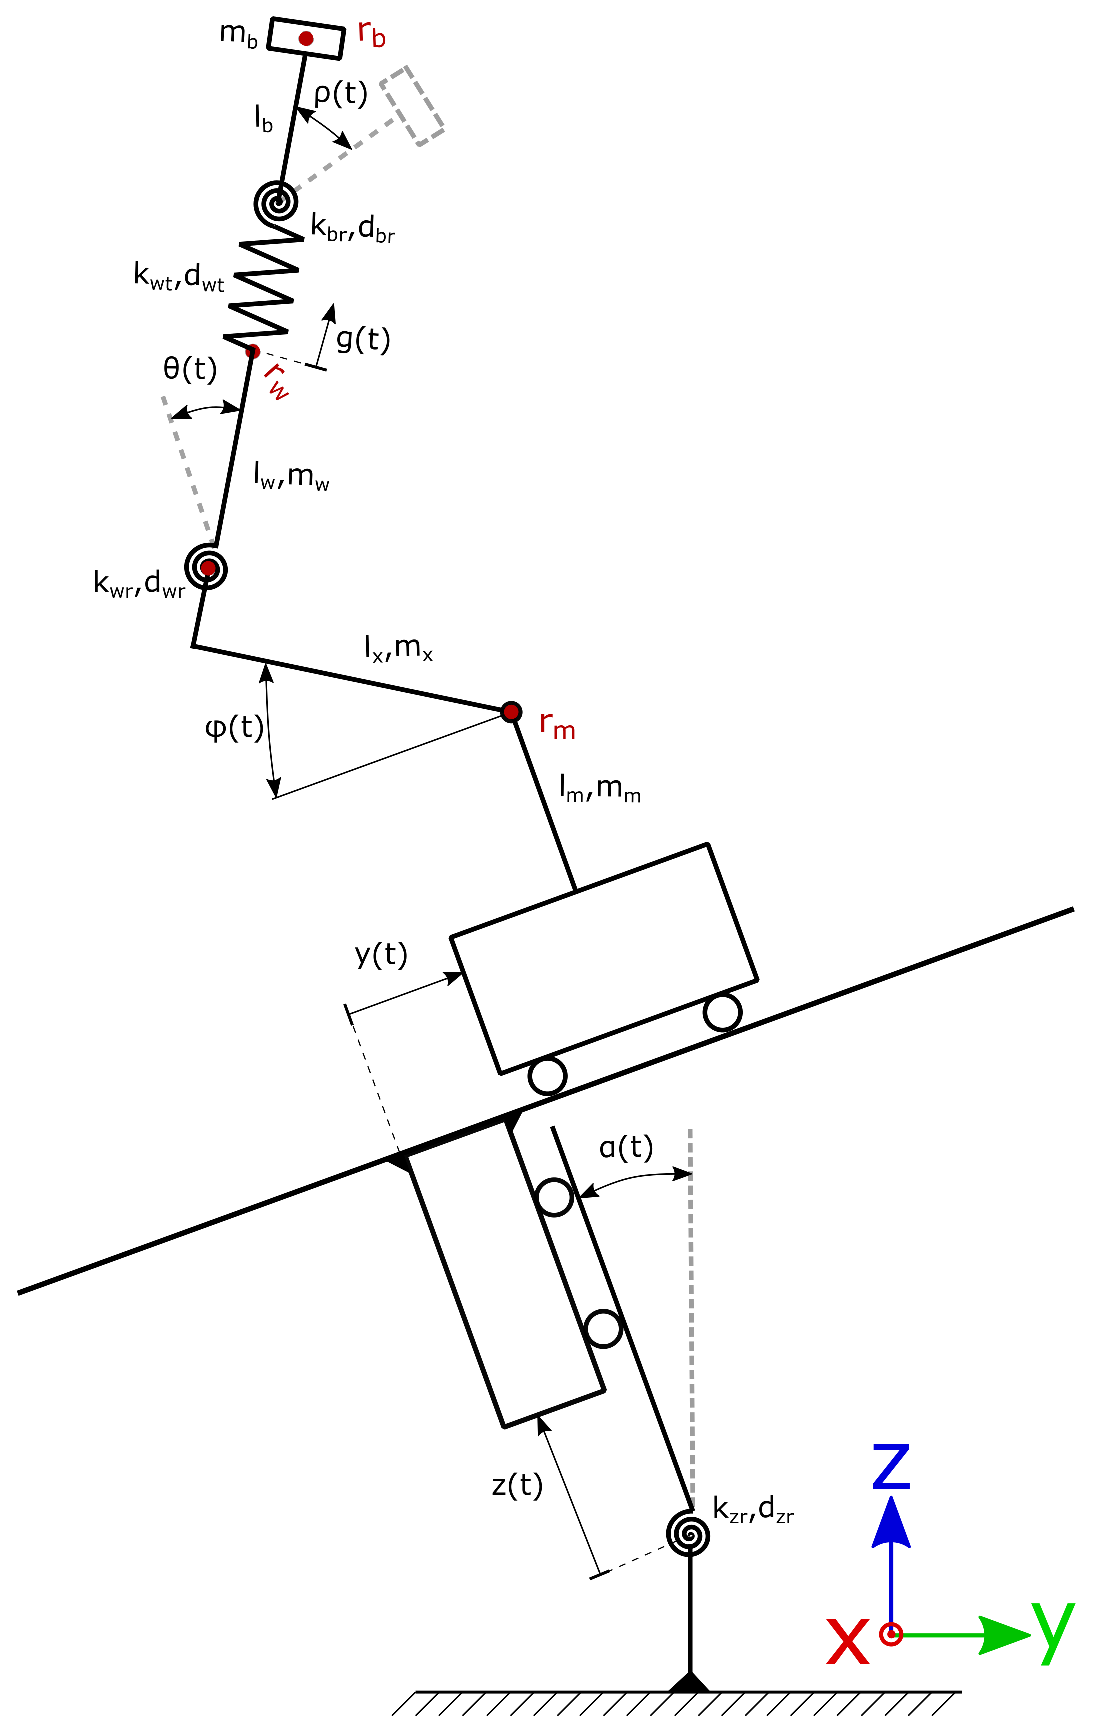
\includegraphics[width=1\linewidth]{./pics/SchematischesModell.eps}
			\end{figure}
		\end{minipage}
		\end{frame}

	\subsection{Auswahl charakteristischer Federsteifigkeiten}
		\begin{frame}
			\includegraphics[width=\linewidth,page=10]{./pics/swarovski.pdf}
		\end{frame}

		\begin{frame}{\small Berücksichtigung charakteristischer Federsteifigkeiten}
                          \textbf{\color{umitblau}Auslenkung Bodyholder infolge externer Kraft} 
					\begin{align*}
					k_{Mx} &= 34.9\frac{kNm}{rad}, F_{ext}=20N, l=0.075m, r=0.0286m\\
					M_{ext} &= 0.075\cdot20 = 1.5Nm, \quad \rho = \frac{M_{ext}}{k_{Mx}} = 42\mu rad\\
					\Delta z &= \rho\cdot l=\bm{3.15\mu m}\quad \Delta y=\rho\cdot r=\bm{1.20\mu m}
					\end{align*}
                  \begin{columns}[totalwidth=\textwidth]
			\begin{column}{0.7\textwidth}
                          \textbf{\color{umitblau}Auslenkung Bodyholder infolge Trägheit} 
                                        \begin{align*}
                                          M_g &=m_b\cdot g \cdot r =6.7\text{Nmm},\quad \rho = \frac{M_{g}}{k_{Mx}} = 0.193\mu rad\\
                                          \Delta y&=\rho\cdot r=\bm{5.52 n m}
                                        \end{align*}
                                      \end{column}
			\hfill
			\begin{column}{0.28\textwidth}
				\begin{figure}
					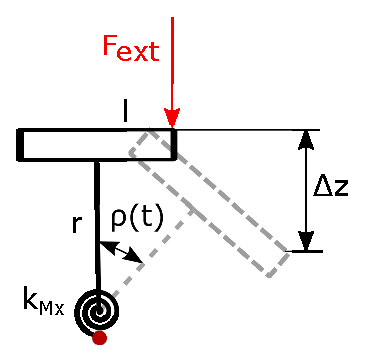
\includegraphics[width=0.6\linewidth]{./pics/bodyHolder.eps}
				\end{figure}
			\end{column}
                      \end{columns}
                          \textbf{\color{umitblau}Eigenfrequenz} 
                          \begin{align*}                                         					f_{0} &= \bm{5687.2 Hz} \quad \text{ mit leichtem Bodyholder } m_b=0.024kg
                          \end{align*}
		\end{frame}

		
		\begin{frame}{\small Berücksichtigung charakteristischer Federsteifigkeiten}
			\begin{minipage}{0.7\textwidth}
				\begin{itemize}
					\item Axialkraft Bodyholder (Konussteifigkeit)
					\begin{align*}
					k_{Fz} &= 6069\frac{kN}{m}, \quad F_{ext}=20N,\quad \Delta z = \frac{F_{ext}}{k_{Fz}} = \bm{3.3\mu m}\\
					\bm{f_{0}} &= \bm{2515.4 Hz} \quad \text{ mit leichtem Bodyholder } 0.024kg 
					\end{align*}
					\item Verkippung RotBody-Achse (ausschließlich aufgrund der Lagersteifigkeit, Welle selbst als Starrkörper angenommen)
					\begin{align*}
					k_{Mx} &= 217.19\frac{kNm}{rad}, \quad F_{ext}=20N, \quad l=0.06m\\
					M_{ext} &= 0.06\cdot20 = 1.2Nm,\quad \theta = \frac{M_{ext}}{k_{Mx}} = 5.525\mu rad\\
					\Delta y &= \theta\cdot l=\bm{0.33\mu m}\\ 
					f_{0} &= \bm{516.5 Hz} \text{ ohne Bodyholder}
					\end{align*}
					
				\end{itemize}
			\end{minipage}
			\hfill
			\begin{minipage}{0.28\textwidth}
				\begin{figure}
					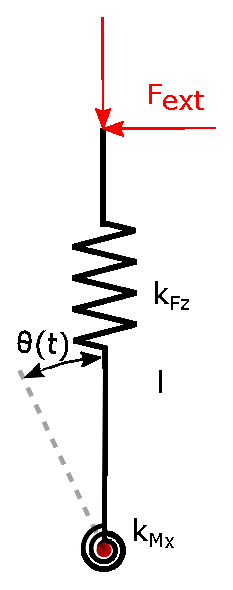
\includegraphics[width=0.4\linewidth]{./pics/rotBody.eps}\\\vspace{0.5cm}
				\end{figure}
			\end{minipage}
		\end{frame}
	
		\begin{frame}{\small Berücksichtigung charakteristischer Federsteifigkeiten}
		\begin{minipage}{0.7\textwidth}
			\begin{itemize}
				\item Biegung RotX-Achse
				\begin{align*}
				k_{Mx} &= 315\frac{kNm}{rad}, \quad F_{ext}=20N, \quad l=0.079m\\
				M_{ext} &= 0.079\cdot20 = 1.58Nm\\
				\varphi &= \frac{M_{ext}}{k_{Mx}} = 5\mu rad\\
				\Delta y &= \theta\cdot l=\bm{0.396\mu m}\\
				f_{0} &= \bm{543.9 Hz} \quad \text{nur mit Masse } m_{x} \text{ ohne } m_{w}, m_{b}  
				\end{align*}
				\item RotX Axialkraft
				\begin{align*}
				k_{Fy} &= 57597\frac{kN}{m}, \quad F_{ext}=20N\\
				\Delta y &= \frac{F_{ext}}{k_{Fy}} = \bm{0.35\mu m}\\
				f_{0} &= \bm{547.34 Hz} \quad \text{ebenfalls nur mit Masse } m_{x}  
				\end{align*}
			\end{itemize}
		\end{minipage}
		\hfill
		\begin{minipage}{0.28\textwidth}
			\begin{figure}[t]
				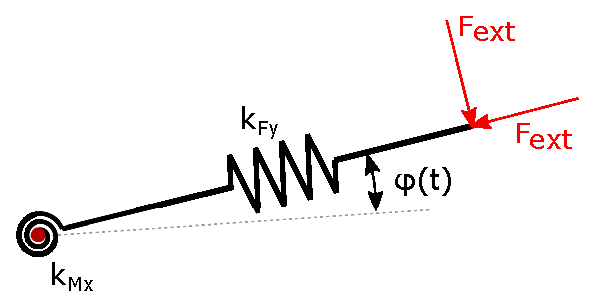
\includegraphics[width=1\linewidth]{./pics/rotX.eps}
			\end{figure}
		\end{minipage}
		\end{frame}

\section{Herleitung der Bewegungsgleichungen}
	\begin{frame}
		Aufstellen der kinetischen und den potentiellen Energien
		\begin{align*}
			T_{t}&= \frac{1}{2}\bigg(m_{m}v_{com_{m}}^{2} +m_{d}v_{com_{d}}^{2}+m_{w}v_{com_{w}}^{2}+m_{b}v_{com_{b}}^{2}\bigg)\\  
			T_{r}&= \frac{1}{2}\bigg(J_{z}\dot{\alpha}^{2}+J_{x}(\dot{\alpha}+\dot{\varphi})^{2} +J_{w}(\dot{\alpha}+\dot{\varphi}+\dot{\theta})^{2} +J_{b}(\dot{\alpha}+\dot{\varphi}+\dot{\theta}+ \dot{\rho})^{2}\bigg)\\   
			U_{t} &= \frac{1}{2}k_{wt}g(t)^{2}\\
			U_{r} &= \frac{1}{2}\bigg(k_{zr}\alpha(t)^{2}+ k_{wr}\theta(t)^{2}+k_{br}\rho(t)^2\bigg)\\
		\end{align*}
		Lagrange-Gleichung
		\begin{equation*}
			L = T_{t}+T_{r} - (U_{t}+U_{r})
		\end{equation*}
		Dissipationsfunktionen:
		\begin{align*}
		D_{t} &= \frac{1}{2}d_{wt}\dot{g}(t)^{2}, \quad
		D_{r} = \frac{1}{2}\bigg(d_{zr}\dot{\alpha}(t)^{2} + d_{wr}\dot{\theta}(t)^{2} + d_{br}\dot{\rho}(t)^{2}\bigg)\\
		D_{ges} &= D_{t} + D_{r}\\
		\end{align*}
	\end{frame}

	\begin{frame}
		Generalisierte Kräfte:
		\begin{align*}
			Q & = [F_{y}, F_{z}, M_{\varphi},0 , 0, 0, 0]^{T}
		\end{align*}
		Lagrange Gleichung 2. Art:
		\[\frac{d}{dt}\bigg(\frac{\partial L}{\partial \bm{\dot{q}}} \bigg) -\frac{\partial L}{\partial \bm{q}} + \frac{\partial D_{ges}}{\partial \bm{\dot{q}}} = Q \]
		\begin{align*}
			M = \frac{\partial}{\partial\bm{\dot{q}}}\frac{\partial L}{\partial\bm{\dot{q}}}, \quad 
			C = \frac{\partial}{\partial\bm{q}}\frac{\partial L}{\partial\bm{\dot{q}}}, \quad
			F = \frac{\partial L}{\partial\bm{q}}, \quad 
			D = \frac{\partial D}{\partial\bm{\dot{q}}} \\
		\end{align*}
		\[ M\bm{\ddot{q}} + C\bm{\dot{q}} - F = Q - D\]
		\begin{equation*}
			\Rightarrow \bm{\ddot{q}}=  - M^{-1}C\bm{\dot{q}} + M^{-1}F + M^{-1}Q - M^{-1}D
		\end{equation*}
		\begin{itemize}
			\item Zur Simulation des Systems werden die Bewegungsdifferentialgleichungen in Form von DGL 1. Ordnung übergeben 
		\end{itemize}
	\end{frame}

\section{Vorwärtskinematik}
	\begin{frame}{Vorwärtskinematik}
		\begin{itemize}
			\item Ziel: Darstellung der Position des Bodies
		\end{itemize}
		Transformationsmatrizen
		\begin{align*}
			T_{0y} &= \begin{bmatrix}\cos\alpha & -\sin\alpha & 0\\\sin\alpha & \cos\alpha & z_{Feder}\\0&0&1 \end{bmatrix}, \quad
			T_{ym} = \begin{bmatrix}-\cos\varphi & \sin\varphi & y(t)+rx_{y0}\\\sin\varphi & \cos\varphi & z(t)+rx_{z0}\\0&0&1 \end{bmatrix}\\
			T_{mw} &= \begin{bmatrix}\cos(\theta) & -\sin(\theta) & lx_{y}\\\sin(\theta) & \cos(\theta) & lx_{z}\\0&0&1 \end{bmatrix}, \qquad
			T_{wb} = \begin{bmatrix}\cos\rho & -\sin\rho & dy\\\sin\rho & \cos\rho & l_{w}+g(t)+l_{b}\\0&0&1 \end{bmatrix}\\
			T_{0b}&= T_{0y}\cdot T_{ym}\cdot T_{mw}\cdot T_{wb}
		\end{align*}
		Ausgangspunkt: Ursprung $ \bm{r_{0}} = [0, 0]^{T} $
		\begin{align*}
			\begin{bmatrix}\bm{r_{b}}\\1\end{bmatrix} = T_{0b}\cdot\begin{bmatrix}\bm{r_{0}}\\1\end{bmatrix}
		\end{align*}
	\end{frame}

\section{Ergebnisse}
	\begin{frame}{Vergleich der Eigenfrequenzen}
		Eigenfrequenzen in Abhängigkeit verschiedener Stellungen der RotX-Achse\\\vspace{0.5cm}
		\begin{minipage}{0.48\textwidth}
			\centering
			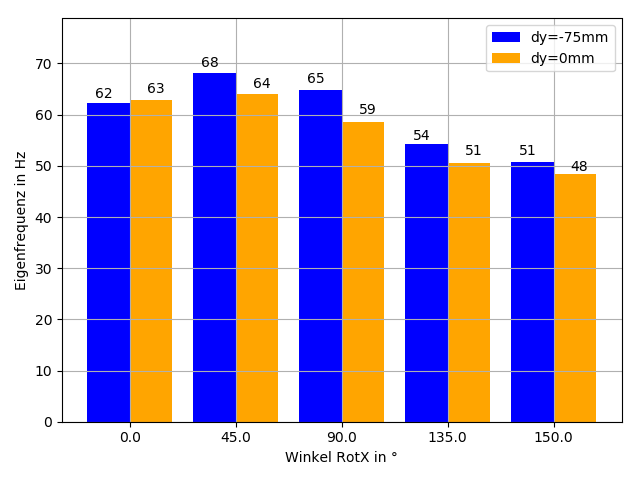
\includegraphics[width=0.99\linewidth]{./pics/eigenfreq_test.png}
			Simulation
		\end{minipage}
		\hfill
		\begin{minipage}{0.48\textwidth}
			\centering
			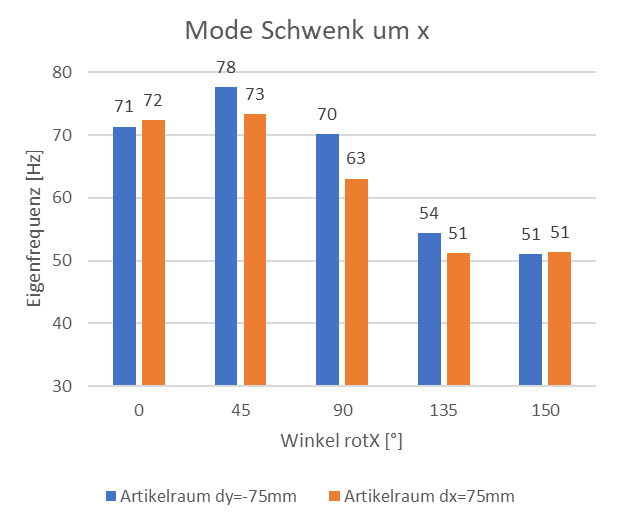
\includegraphics[width=0.99\linewidth]{./pics/eigenfreq_ref.png}
			FEM-Simulation
		\end{minipage}
	\vspace{0.5cm}
		\begin{itemize}
			\item Zur Bestimmung der Eigenfrequenzen wurde kein Regler verwendet. Achsen wurden starr ausgelegt.
		\end{itemize}
	\end{frame}

	\begin{frame}{Simulationsszenarien}
		\begin{minipage}{0.58\textwidth}
			\textbf{Gilt für alle Simulationsszenarien}
			\begin{itemize}
				\item Simulationszeit: $ t_{0} = 0, \quad T = 400ms $
				\item Bewegungsdauer: $ 200ms $
				\item Ausgangs- und Zielposition sind identisch. Die Orientierung der RotX-Achse wird jedoch geändert.
					\begin{align*}
					ee(t) &= [y(t), z(t), \varphi(t)]\\
					ee(t=0) &= [0.04m,0.826m,90^{\circ}]\\
					ee(t=T) &= [0.04m,0.826m,0^{\circ}]
					\end{align*}	
				\item PID Regler für jede Achskoordinate (sehr steif ausgelegt)
				\item Regelung mit Vorsteuerung und computed torque
				\item Vorgabe Bestückposition und -orientierung für $ t_{0} $ und $ T $, Umrechnung und Bahnplanung in Gelenkskoordinaten
			\end{itemize}
		\end{minipage}	
		\hfill
		\begin{minipage}{0.39\textwidth}
			\vspace{-0.2cm}
			\begin{figure}
				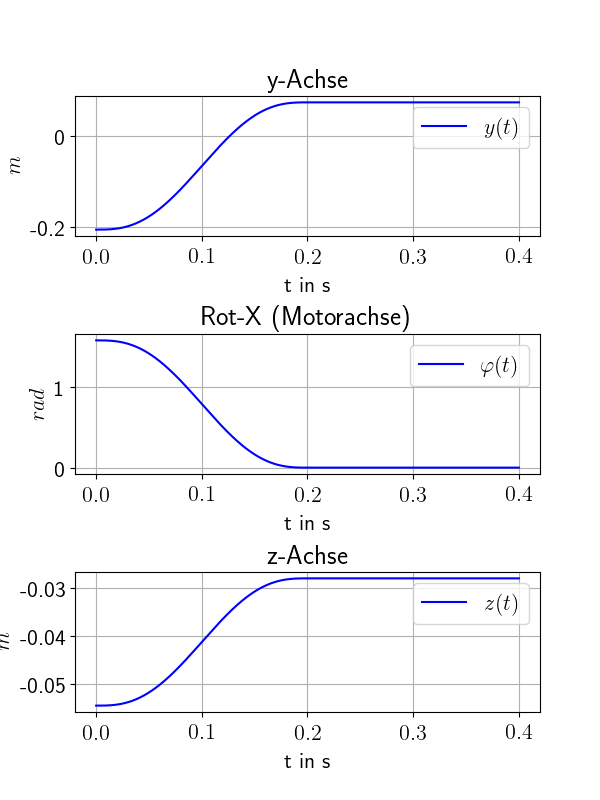
\includegraphics[width=1.1\linewidth]{./pics/input_starr.png}
			\end{figure}
		\end{minipage}
	\end{frame}

	\begin{frame}{Simulationsszenarien}
		\begin{minipage}{0.58\textwidth}
			\textbf{Übersicht der Simulationsszenarien}
			\begin{itemize}
				\item \textcolor{blue!60!black}{Simulation 1:} Starres System
				\item \textcolor{blue!60!black}{Simulation 2:} Nur der Unterbau schwingt, restliches System ist starr (nur Biegefeder $ k_{zr} $)
				\item \textcolor{blue!60!black}{Simulation 3:} Unterbau und RotBody-Achse sind schwingungsfähig (Biegefedern $ k_{zr} $ und $ k_{wr} $)
				\item \textcolor{blue!60!black}{Simulation 4:} Vorsteuerung mit Input-shaping	
		\end{itemize}
		\end{minipage}
		\hfill
		\begin{minipage}{0.38\textwidth}
			\begin{figure}
				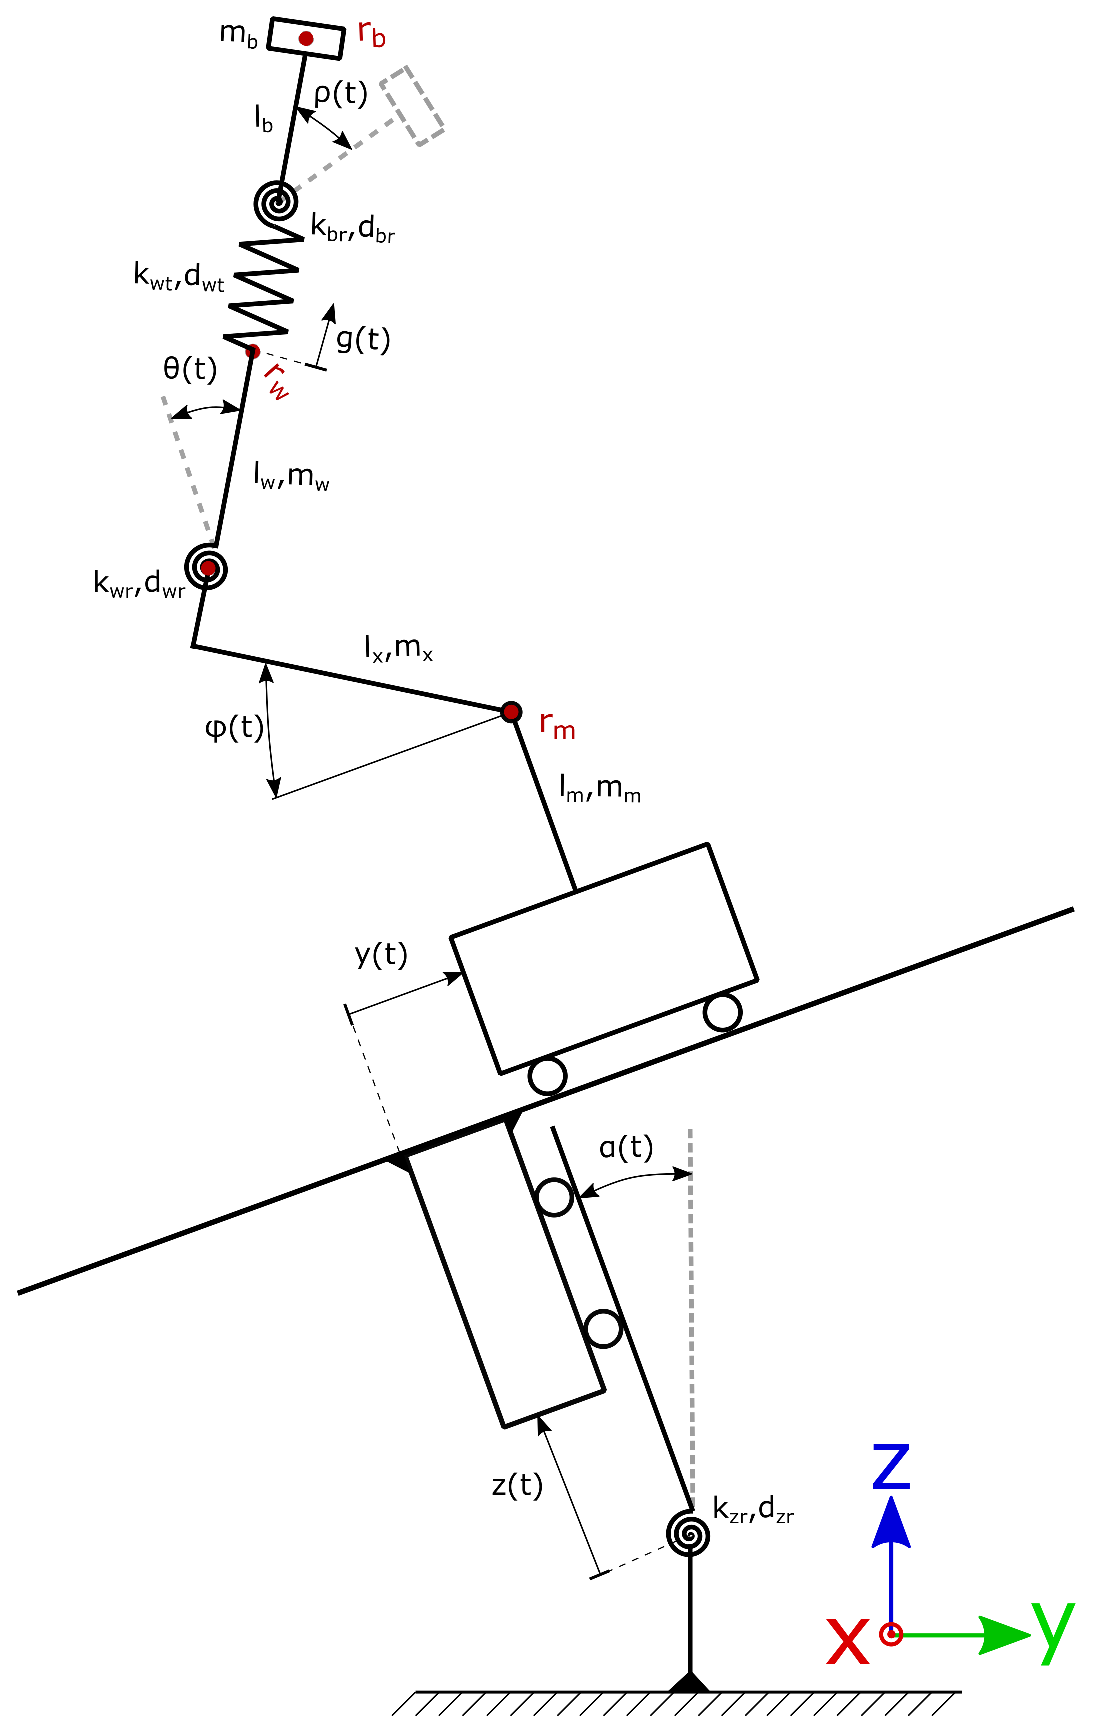
\includegraphics[width=1.1\linewidth]{./pics/SchematischesModell.eps}
			\end{figure}
		\end{minipage}		
	\end{frame}

	\begin{frame}{Simulation 1 - starres System}
		Fehlergrößenverlauf für die Simulation des starren Systems
		\vspace{-0.2cm}
		\begin{figure}
			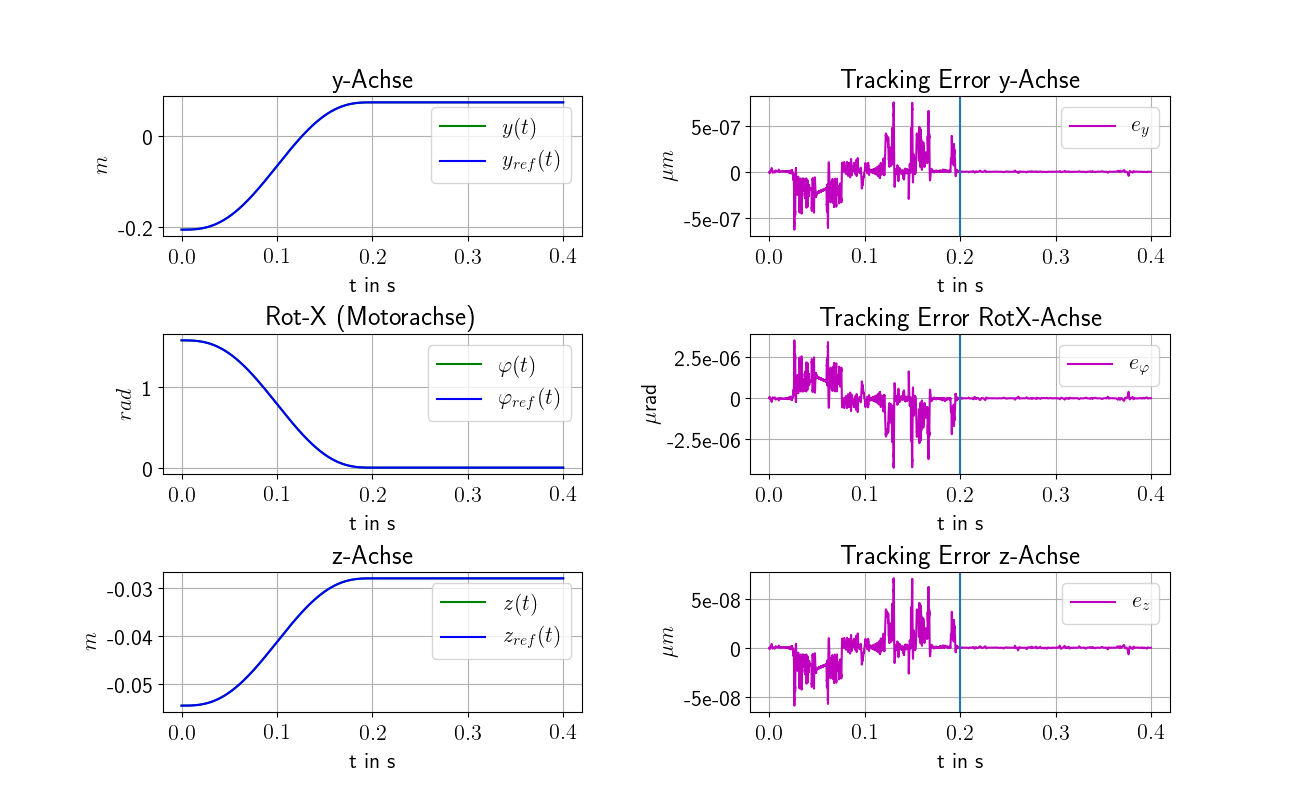
\includegraphics[width=0.99\linewidth]{./pics/posVerlaufAchsen_starr.png}
		\end{figure}
	\end{frame}

	\begin{frame}{Simulation 1 - starres System}
		Bahnverlauf des Bestückpunktes in der Ebene (links), Fehlerverlauf der Bestückposition und -orientierung zur Referenzbahn (rechts)
		\vspace{-0.2cm}
		\begin{figure}
			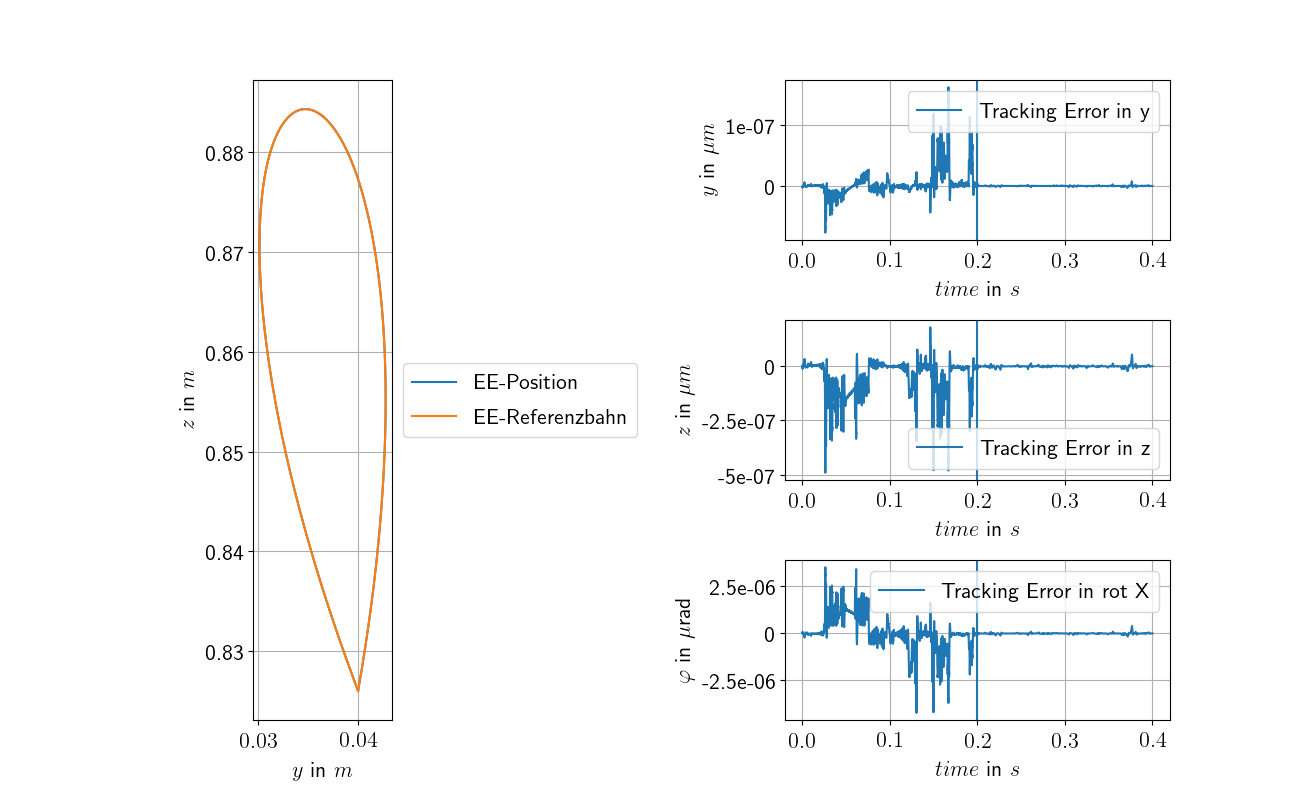
\includegraphics[width=0.999\linewidth]{./pics/endeffektor_starr.png}
		\end{figure}
	\end{frame}

	\begin{frame}{Simulation 2 - schwingender Unterbau}
		Fehlergrößenverlauf für die Simulation mit schwingendem Unterbau durch die Biegefeder $ k_{zr} $
		\vspace{-0.2cm}
		\begin{figure}
			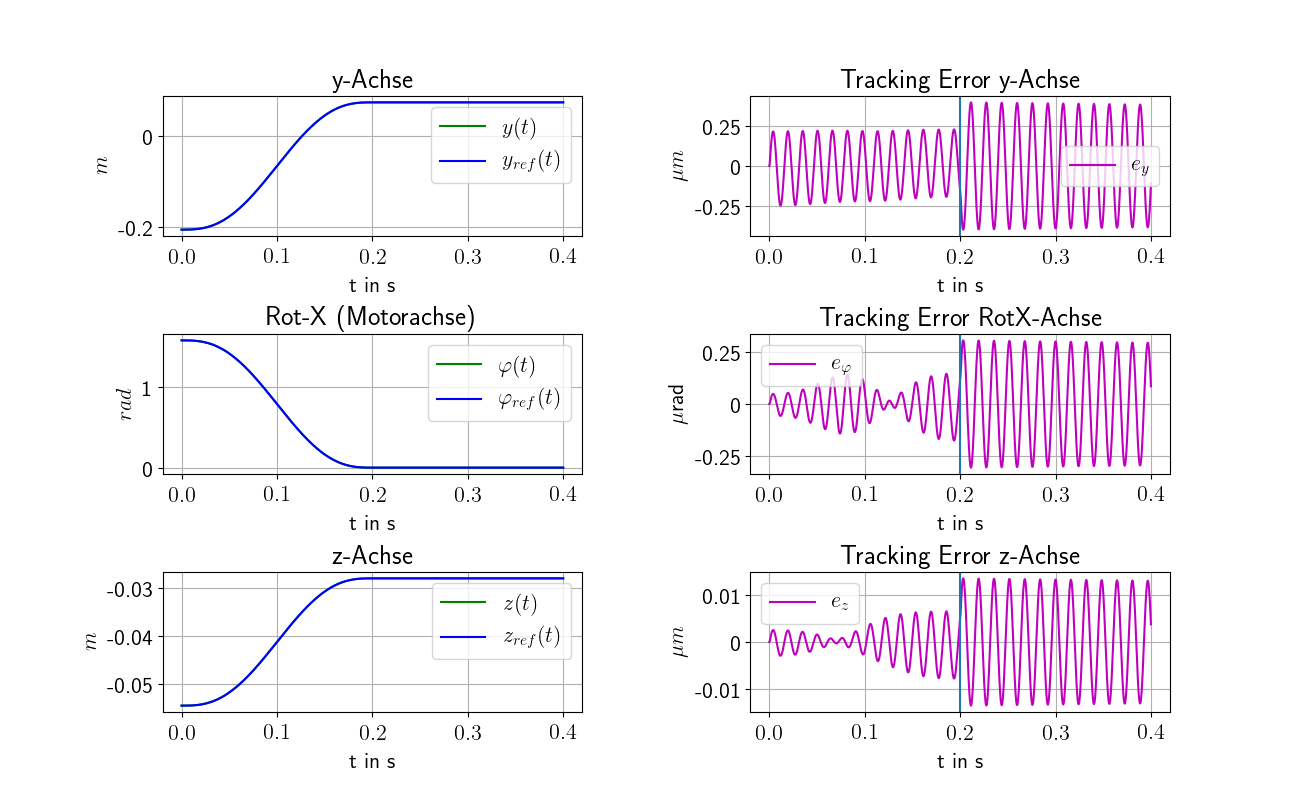
\includegraphics[width=0.99\linewidth]{./pics/posVerlaufAchsen_nurZ.png}
		\end{figure}
	\end{frame}

	\begin{frame}{Simulation 2 - schwingender Unterbau}
		Bahnverlauf des Bestückpunktes in der Ebene (links), Fehlerverlauf der Bestückposition und -orientierung zur Referenzbahn (rechts)
		\vspace{-0.2cm}
		\begin{figure}
		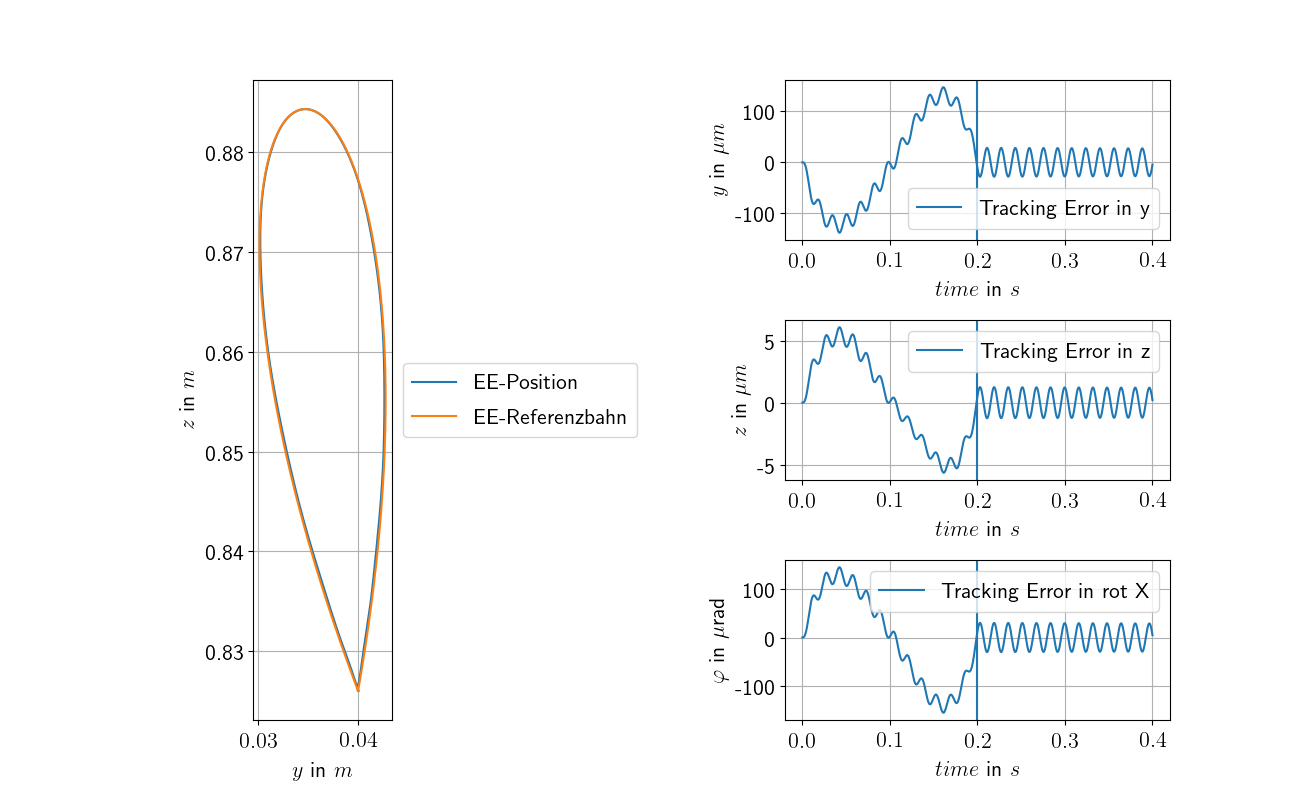
\includegraphics[width=0.999\linewidth]{./pics/endeffektor_nurZ.png}
		\end{figure}
	\end{frame}

	\begin{frame}{Simulation 3}
		Fehlergrößenverlauf für die Simulation mit schwingendem Unterbau und schwingender RotBody-Achse
		\vspace{-0.2cm}
		\begin{figure}
			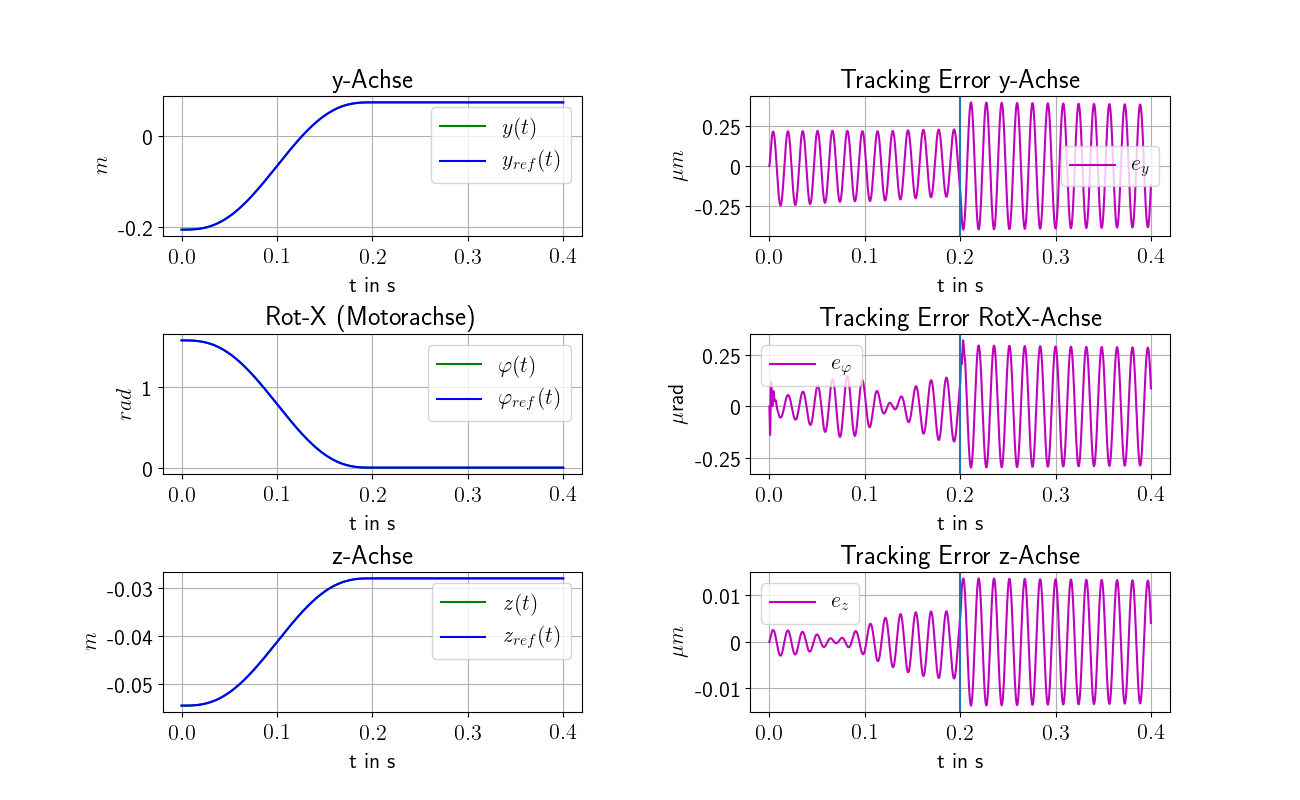
\includegraphics[width=0.99\linewidth]{./pics/posVerlaufAchsen_ZundTheta.png}
		\end{figure}
	\end{frame}

	\begin{frame}{Simulation 3}
		Bahnverlauf des Bestückpunktes in der Ebene (links), Fehlerverlauf der Bestückposition und -orientierung zur Referenzbahn (rechts)
		\vspace{-0.2cm}
		\begin{figure}
		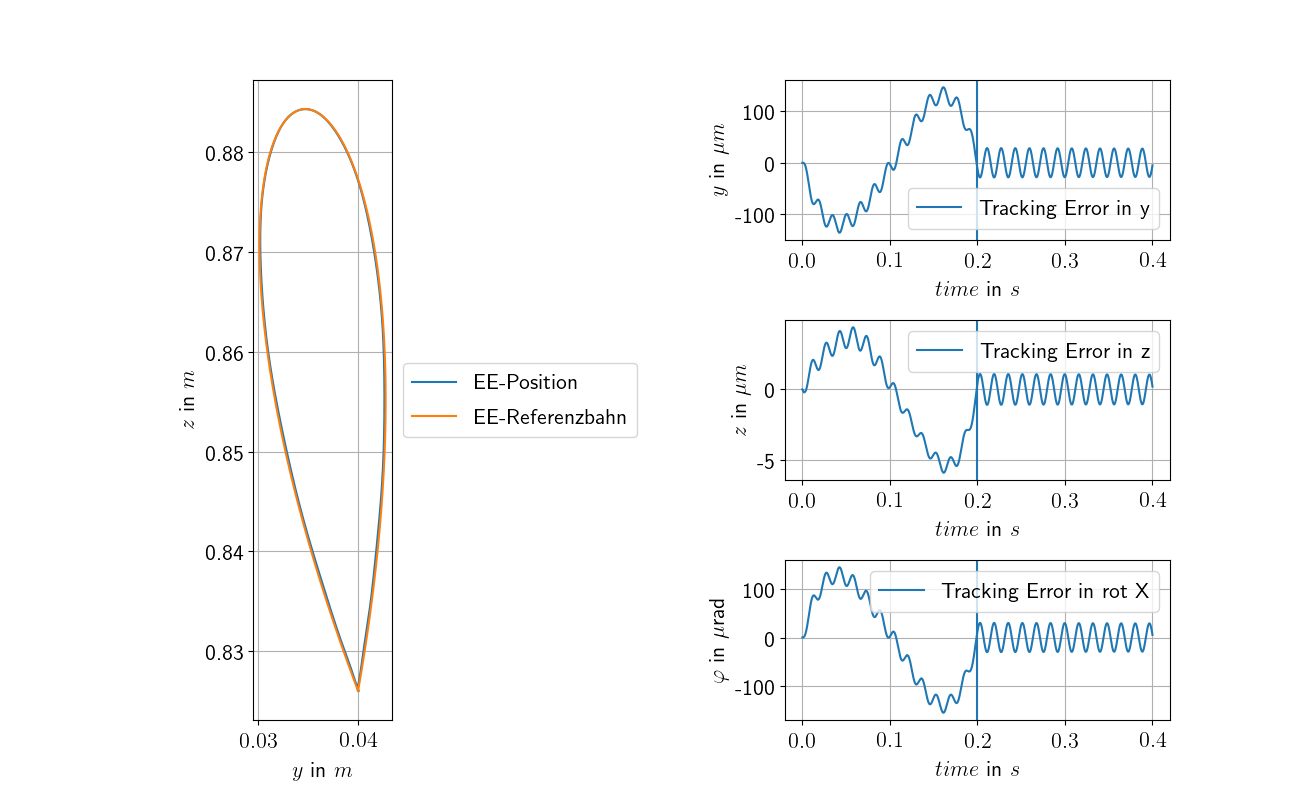
\includegraphics[width=0.999\linewidth]{./pics/endeffektor_ZundTheta.png}
		\end{figure}
	\end{frame}

	\begin{frame}{Simulation 4 - Vorsteuerung mit Input-shaping}
		Fehlergrößenverlauf für die Simulation mit schwingendem Unterbau und schwingender RotBody-Achse
		\vspace{-0.2cm}
		\begin{figure}
			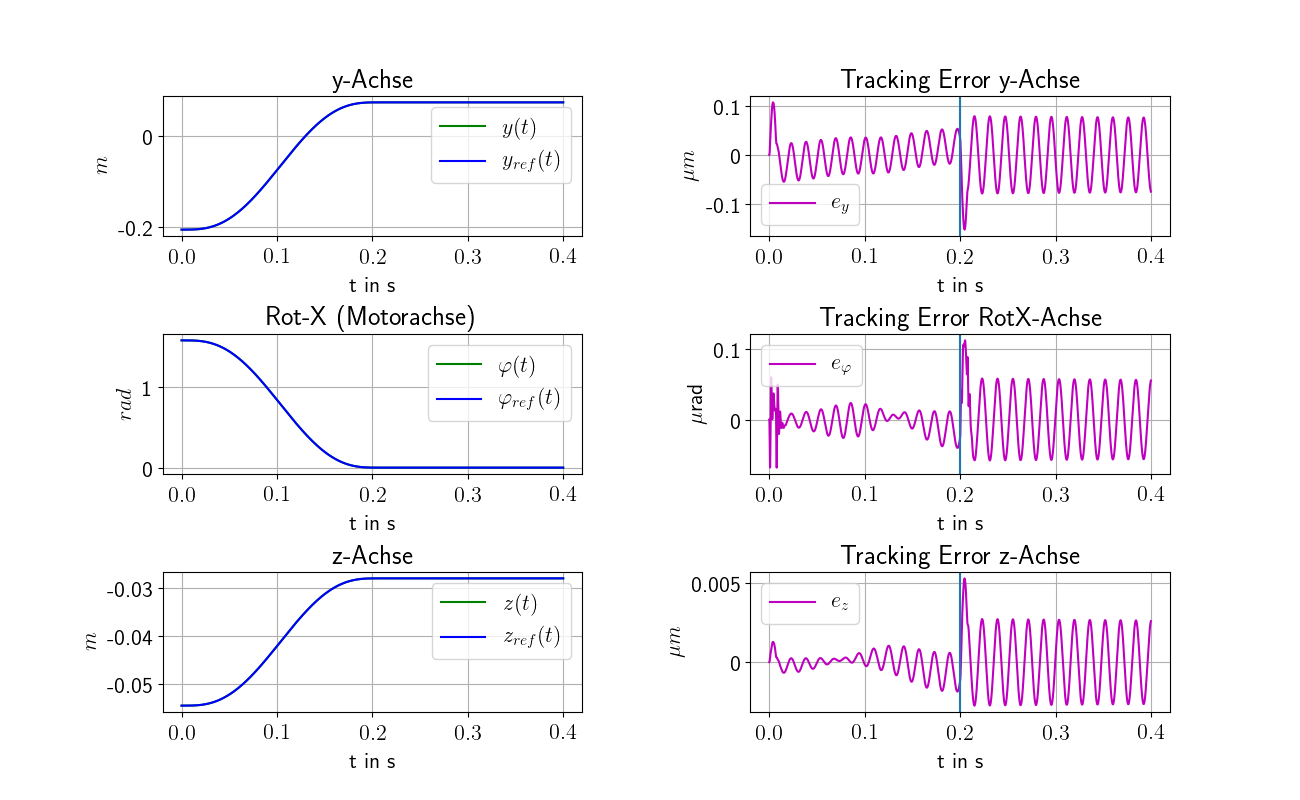
\includegraphics[width=0.99\linewidth]{./pics/posVerlaufAchsen_shift.png}
		\end{figure}
	\end{frame}

	\begin{frame}{Simulation 4 - Vorsteuerung mit Input-shaping}
	\vspace{-0.1cm}
		Bahnverlauf des Bestückpunktes in der Ebene (links), Fehlerverlauf der Bestückposition und -orientierung zur Referenzbahn (rechts)
		\vspace{-0.2cm}
		\begin{figure}
		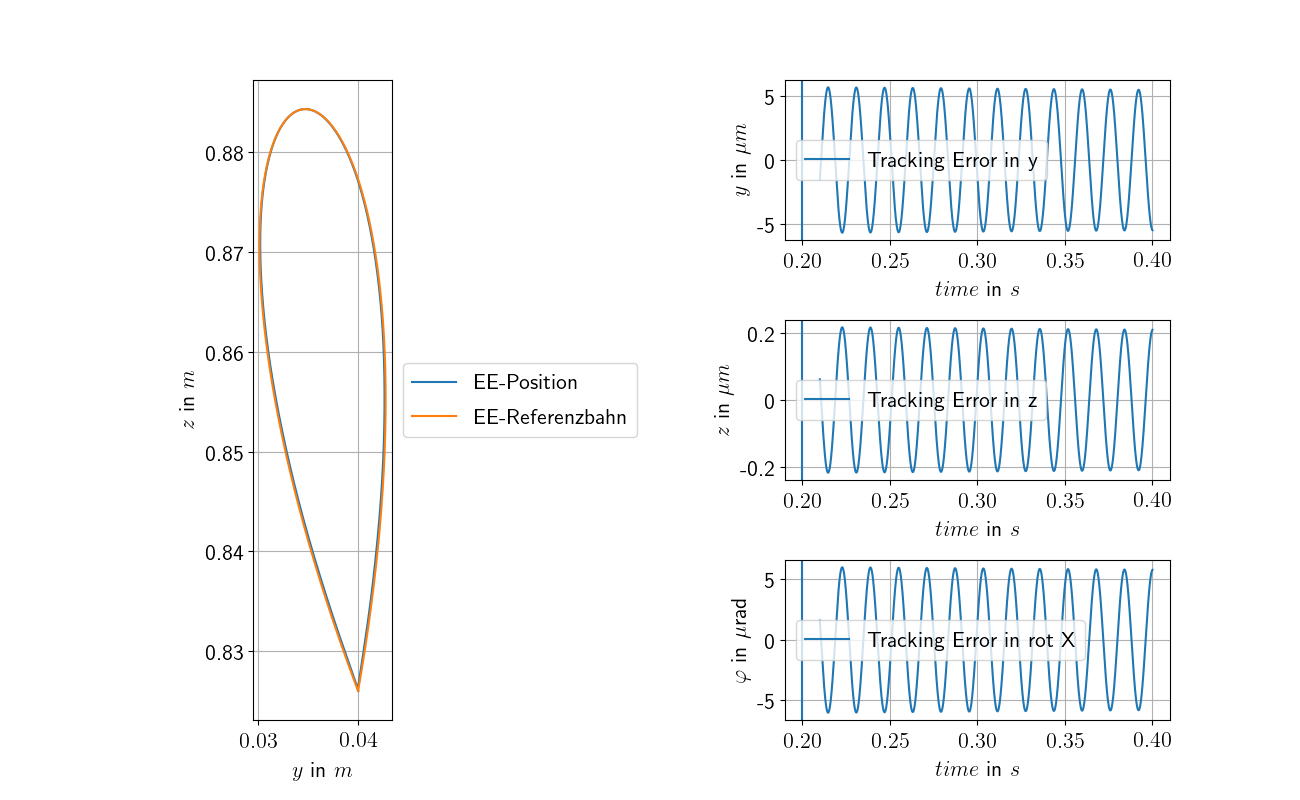
\includegraphics[width=0.9\linewidth]{./pics/endeffektorZoom_shift.png}
		\end{figure}
		\begin{itemize}
			\item $ 10Hz $ Fehler an Eigenfrequenz
		\end{itemize}
	\end{frame}

\section{Verbesserungen des Modells}
	\begin{frame}{\small Berücksichtigung der Steifigkeits-Deviationsanteile}
		\begin{minipage}{0.68\textwidth}
			\textbf{Problem:}
			\begin{itemize}
				\item Deviationsanteile der Steifigkeitsmatrix sind für die Rot-Body-Achse nicht vernachlässigbar
			\end{itemize}
			\textbf{Lösung:}
			\begin{itemize}
				\item Annahme: Für das dynamische Verhalten sind die einwirkenden Momente sehr gering
				\item Idee: Verformung durch nur eine Drehfeder abbilden, wobei die Position und die Steifigkeit der Feder so gewählt wird, dass das gewünschte Verhalten erreicht wird  
				\item 2. Schritt: Abstimmung der beiden Stäbe auf die Gesamtmasse, Gesamtlänge, resultierender Schwerpunkt und Eigenfrequenz 
			\end{itemize}
		\end{minipage}
		\hfill
		\begin{minipage}{0.3\textwidth}
			\begin{figure}
				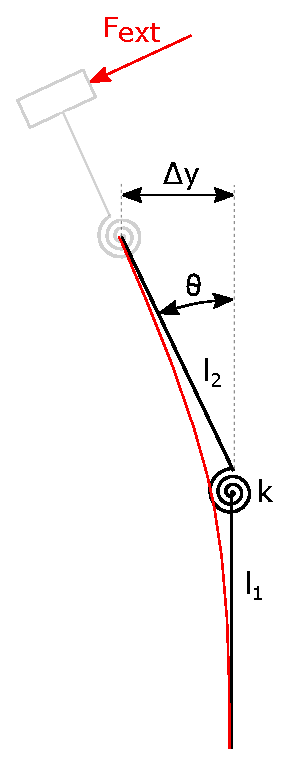
\includegraphics[width=0.7\linewidth]{./pics/rotBody_idea.eps}
			\end{figure}
		\end{minipage}
		
	\end{frame}

\section{Next Steps}
	\begin{frame}{Next Steps}
		\textbf{Die nächsten sinnvollen Schritte vom jetzigen Stand des Modells aus:}
		\begin{enumerate}
			\item Elektrischer Teil des Motormodells implementieren
			\item Daten für Spindelantrieb berücksichtigen (Steigung, Gesamtübersetzung)
			\item Parameteridentifikation am Aufbau
		\end{enumerate}
	\end{frame}

%\section{Offene Fragen}
%	\begin{frame}{Offene Fragen}
%	\textbf{Unklarheiten der FEM-Simulationen}
%	\begin{enumerate}
%		\item Fersteifigkeit RotBody-Welle nur in Kombination mit Konussteifigkeit und Lagersteifigkeit verfügbar?
%	\end{enumerate}
%	\end{frame}

\end{document}


